\documentclass[a4paper,12pt]{article}

% Зачеркивание
\usepackage{cancel}

% Работа с русским языком
\usepackage{cmap}					% Поиск в PDF
\usepackage[T2A]{fontenc}			% Кодировка
\usepackage[utf8]{inputenc}			% Кодировка исходного текста
\usepackage[english,russian]{babel}	% Языки и переносы

% Правила переноса
\usepackage{hyphenat}
\hyphenation{ма-те-ма-ти-ка вос-ста-нав-ли-вать}

% Размеры страниц и отступы
\usepackage[a4paper,top=2cm,bottom=2cm,left=3cm,right=1.5cm]{geometry}
% \linespread{1.5}

% Дополнительная работа с математикой
\usepackage{amsmath,amsfonts,amssymb,amsthm,mathtools, mathtext, cite, enumerate, float} % Пакеты АМО
\usepackage{icomma} % "Умная" запятая: $0,2$ --- число, $0, 2$ --- перечисление
\usepackage{gensymb}
\newcommand{\expnumber}[2]{{#1}\mathrm{e}{#2}} % Для записи 1e-4

% Шрифты
\usepackage{euscript}	 % Шрифт Евклид
\usepackage{mathrsfs} % Красивый матшрифт

% Перенос знаков в формулах (по Львовскому)
\newcommand*{\hm}[1]{#1\nobreak\discretionary{}
{\hbox{$\mathsurround=0pt #1$}}{}}

% Работа с картинками
\usepackage{graphicx}  % Для вставки рисунков
\graphicspath{images/}  % Папка с рисунками
\setlength\fboxsep{3pt} % Отступ рамки от рисунка
\setlength\fboxrule{1pt} % Толщина линий рамки
\usepackage{wrapfig} % Обтекание рисунков и таблиц текстом
\usepackage{subfig}
\captionsetup[subfigure]{labelformat=empty}
\usepackage[font={small,it}]{caption}

% Работа с цветами
\usepackage[usenames]{color}
\usepackage{colortbl}

\bibliographystyle{unsrt} % Список источников в порядке упоминания в тексте

% Меняем везде перечисления на цифра.цифра
\renewcommand{\theenumi}{\arabic{enumi}}
\renewcommand{\labelenumi}{\arabic{enumi}}
\renewcommand{\theenumii}{.\arabic{enumii}}
\renewcommand{\labelenumii}{\arabic{enumi}.\arabic{enumii}.}
\renewcommand{\theenumiii}{.\arabic{enumiii}}
\renewcommand{\labelenumiii}{\arabic{enumi}.\arabic{enumii}.\arabic{enumiii}.}


\usepackage{multicol} % Для нескольких уравнений на одной строке

\usepackage[export]{adjustbox} % Для вертикального выравнивания картинки и формулы на одной строке

\usepackage{hyperref} % Для цитирования картинок из интернета

\usepackage[nottoc,numbib]{tocbibind} % Список литературы в содержании

\usepackage{enumitem} % нумерация буквами

% Листинг кода
\usepackage{xcolor}
\usepackage{listings}

\definecolor{mGreen}{rgb}{0,0.6,0}
\definecolor{mGray}{rgb}{0.5,0.5,0.5}
\definecolor{mPurple}{rgb}{0.58,0,0.82}
\definecolor{backgroundColour}{rgb}{0.95,0.95,0.92}

\lstdefinestyle{CStyle}{
    backgroundcolor=\color{backgroundColour},   
    commentstyle=\color{mGreen},
    keywordstyle=\color{magenta},
    numberstyle=\tiny\color{mGray},
    stringstyle=\color{mPurple},
    basicstyle=\footnotesize,
    breakatwhitespace=false,         
    breaklines=true,                 
    captionpos=b,                    
    keepspaces=true,                 
    numbers=left,                    
    numbersep=5pt,                  
    showspaces=false,                
    showstringspaces=false,
    showtabs=false,                  
    tabsize=2,
    language=C
}

\renewcommand{\scriptsize}{\fontsize{14}{14pt}\selectfont}
\renewcommand{\baselinestretch}{1.5}
\usepackage{titlesec}
\titleformat{\section}
{\normalsize\scriptsize\bfseries}
{\thesection}
{1em}{\scriptsize\bfseries}
\titleformat{\subsection}
{\normalsize\scriptsize\bfseries}
{\thesubsection}
{1em}{\scriptsize\bfseries}
\titleformat{\subsubsection}
{\normalsize\scriptsize\bfseries}
{\thesubsubsection}
{1em}{\scriptsize\bfseries}


\begin{document}
\tableofcontents
\newpage

\section{Введение}
\subsection{Зачем нужны промыслово-геофизические исследования}
\par
Промыслово-геофизические мероприятия проводятся для оптимизации процесса разработки месторождения с целью увеличения добычи нефти. ПГИ могут проводиться как при работающей скважине, так и при остановленной. Иногда для сбора достаточного для анализа количества данных проводится несколько исследований на различных этапах работы скважины.
\par
Одна из основных задач ПГИ - локализация зон притока флюида в скважину. Как правило, при этом решается еще и задача определения типа флюида - вода, нефть, газ или смесь флюидов - и определение характеристик флюида - плотность и скорость.
\par
Одно из наиболее эффективных мероприятий для увеличения добычи углеводородов - проведение многостадийного гидроразрыва пласта \cite{fracking}. В скважину под большим давлением (до 100МПа) закачивается жидкость разрыва высокой вязкости (на водной или нефтяной основе). Под влиянием давления жидкости разрыва пласт расщепляется. После этого в скважину закачивается жидкость-песконоситель при давлении, позволяющем удержать скважину в открытом состоянии. Жидкость-песконоситель - более вязкая, чем жидкость разрыва, и содержит проппант - песок или другие гранулы диаметром обычно порядка 0.5-1.2мм. Шарики проппанта затекают в образовавшиеся трещины. При откачке жидкости давление снижается, но образовавшиеся трещины не схлопываются полностью из-за наличия в них шариков проппанта, при этом часть проппанта разрушается, а часть вдавливается в породу. Раскрытые трещины позволяют значительно увеличить прирост нефти.

ПГИ могут проводиться при проведении многостадийного гидроразрыва пласта \cite{191562}. Анализ данных ПГИ позволяет оценить качество полученных трещин и локализовать зоны притоков в скважине.
\par
Другая часто решаемая задача - поиск неисправностей в структуре скважины, то есть нежелательных трещин, или утечек \cite{204557}.

\subsection{Оборудование для каротажа}
\par
В ходе ПГИ в скважину опускается каротажная сборка приборов, которая проводится по всей глубине скважины и непрерывно пишет данные. Приборы могут состоять из одного или нескольких датчиков, измеряющих различные физические величины.

\subsubsection{Стандартные датчики}
\par
Часто используемый для ПГИ прибор PLT-9.2 \cite{92} содержит в себе датчики температуры, давления, влагомер и расходомер. Для привязки показаний прибора к траектории скважины используется локатор муфт и датчик уровня естественного гамма-излучения \cite{169255}.

\subsubsection{Акустическая шумометрия}
\par
В рамках измерения спектральный шумомер записывает акустические сигналы в скважине в широком диапазоне частот с хорошим разрешением: анализируемые в данной работе данные пассивной акустической шумометрии были получены приборами с диапазоном измерений от 8Гц до 60кГц и от 8Гц до 100кГц, записанными в 512 или 1024 частотных каналов с высокой чувствительностью. Каждой точке траектории, в которой производились измерения, сопоставляется запись акустического шума порядка 0.1сек с частотой дискретизации 200кГц, которая для анализа обычно преобразуется в вектор, компоненты которого соответствуют интенсивности сигнала в определенном диапазоне частот. Запись показаний прибора может проводиться как при движении прибора, так и на остановках (например, каждые 2 метра) - чтобы избежать дорожного шума, который может скрыть низкочастотные сигналы малой интенсивности.
\par
Акустический шум появляется при турбулентном движении флюида по стволу скважины.. Согласно \cite{lighthill}, \cite{191562}, мощность акустического излучения W при таком движении зависит от параметров трубы и флюида:
\begin{equation}
\label{eq:power_law}
    W\sim\frac{\rho U^8 d^2}{a_0^5},
\end{equation}
Где $\rho$ – средняя по сечению трубы плотность флюида, $a_0$ – скорость звука во флюиде, $U$ – скорость потока и $d$ – диаметр трубы, который задает характерный масштаб турбулентности.
\par
Так как мощность зависит от скорости в восьмой степени, шумометрия - очень чувствительный способ измерения скорости потока. Это позволяет достичь хороших результатов в случае однофазного течения; в случае смеси флюидов меняются и другие компоненты формулы \eqref{eq:power_law} - плотность флюида и скорость звука во флюиде, поэтому показания шумометрии нужно рассматривать в комбинации с остальными показаниями датчиков.
\par
Показано \cite{pa_good}, \cite{187909}, что сочетание пассивной акустической шумометрии с классическими приборами геофизических исследований позволяет улучшить результаты анализа данных ПГИ. 
\par
В частности, одно из достоинств спектральной шумометрии заключается в том, что с ее помощью можно выделить и дифференцировать заколонные перетоки - то есть потоки флюида между обсадной колонной и породой, которые невозможно определить с помощью, например, расходомера. Выявление заколонных перетоков важно для проверки технического состояния скважины, определения расположения продуктивных пластов, оценки эффективности гидроразрыва и т.п.
\par
Также чувствительность современных приборов спектральной шумометрии позволяет уловить притоки со скоростями ниже чувствительности обычных расходомеров, которые при таких скоростях просто не раскручиваются. Поэтому акустическая шумометрия особенно важна в горизонтальных и около-горизонтальных малодебитных скважинах.
\par
Последнее время актуальными становятся измерения акустической шумометрии и температуры с использованием оптоволоконных кабелей – технологии DTS (distributed temperature sensing) и DAS (distributed acoustic sensing) \cite{161712}.

\subsection{Анализ данных ПГИ}
\par
Анализ полученных в результате каротажных исследований данных может проводиться как в ручном режиме, так и с использованием написанных экспертами программ. Невозможность непосредственно измерить такие важные показатели, как пористость и плотность пластов, делают очень сложной задачу численного моделирования скважины для решения задачи с высокой точностью, поэтому обычно используется ручной анализ и/или численное моделирование \cite{196955}.
\par
Рассмотрим для примера задачу локализации зон притока с использованием данных спектральной акустической шумометрии.
\par
При наличии данных пассивной акустической шумометрии «ручной» способ анализа данных обычно предполагает построение спектрограммы в смысле изменения спектра сигнала при продвижении вдоль траектории скважины. Изменения спектра сигнала могут указывать на наличие зон притока.
\par
В \cite{187909} описаны способы локализации зон притока в малодебитных горизонтальных скважинах с использованием спектральной акустической шумометрии. Описаны некоторые характеристики спектрограмм, позволяющие выделить события: так, поток флюида через трубу большого диаметра генерирует низкочастотный шум, а через трубу меньшего диаметра - высокочастотный \cite{162081}; также поток через пористую среду генерирует высокочастотный шум, а течение через естественную или искусственно созданную скважину - низкочастотный. Для избавления от статистически не значимого шума, вызванного движением прибора или фоновым шумом скважины, используются различные техники фильтрации шума, например, на основе вейвлет-преобразования \cite{162081}. В целом притоки углеводородов можно выделить по широкому спектру производимого акустического шума.

\subsection{Решаемые в исследовании задачи}
\par
В данной работе рассмотрены две задачи: локализация зон притока в скважину и определение фазового состава флюида по данным термоанемометрии. 
\par
\textit{Задача локализации зон притока} решается на основе задачи выявления событийных участков в скважине. Событийными участками могут быть притоки воды, нефти или газа, а также изменения показаний приборов, связанные с вариацией траектории скважины. Это могут быть удары каротажной сборки приборов о стенки скважин, изменения показаний из-за стыка труб, или, в случае горизонтальных скважин, индикаторы стратификации жидкости не в местах наличия притоков - в частности, могут существовать места скопления воды на вогнутых по отношению к горизонту участках траектории и газовые облака на выпуклых участках. Так как задача разделения участков на зоны притока и зоны стратификации жидкостей, не связанных с притоком, требует дальнейших кропотливых исследований, в том числе учета мнения экспертов, в данной работе она не рассмотрена. 
\par
Тем не менее, как будет показано далее, предложенный для решения задачи выявления событийных участков подход может быть доработан до семейства алгоритмов, решающих больший диапазон задач анализа данных ПГИ, в том числе и задачу локализации зон притока. В частности, предложенный подход может помочь в решении любой проблемы, которую можно свести к задаче классификации - причем как бинарной классификации, так и задачи классификации на несколько классов\cite{ws_multiclass}. В качестве задачи классификации на несколько классов можно привести задачу локализации зон притока с указанием типа притока - вода, нефть или газ; эта же задача может решаться с применением трех моделей бинарной классификации. 
\par
\textit{Задача определения фазового состава флюида вдоль ствола скважины по данным термоанемометрии} решается с помощью анализа геометрической формы циклов термоанемометрического датчика. Форма зависит от типа флюида, где находится датчик во время цикла (12 сек). Показано, что можно использовать два признака геометрии цикла, вычисляемых на основе значений температуры – как фоновой температуры вдоль оси скважины, так и показаний специального распределенного прибора термоанемометрии, – в качестве координат пространства для кластерного анализа. В этих координатах удается разделить точки-циклы на три достаточно отчетливых кластера, соответствующих воде, нефти и газу. Для учета неопределенности разделение проводится с помощью модели смеси гауссовских распределений, позволяющей приписать каждой точке-циклу вероятность принадлежности к тому или иному кластеру. Это дает возможность не только определить для каждой точки наиболее вероятный соответствующий ей тип флюида, но и оценить фазовый состав при предполагаемом наличии смеси флюидов.


\newpage

\section{Часть 1. Локализация зон притока}
\subsection{Актуальность и обоснование выбора темы}
\par
Данных ПГИ и мониторинга скважин встроенными оптоволоконными системами становится все больше, и зачастую на решение поставленных задач не хватает рук экспертов и времени и ресурсов для численного моделирования; ответ нужен «в реальном времени». Требуется разработать надежные системы автоматизированной обработки – как минимум для выполнения основной части рутинной работы, производимой зачастую вручную; и как оптимум – для подготовки вариантов интерпретации данных и рекомендации решений для выработки экспертом окончательных заключений.
\par
Методы машинного обучения могут оказать серьезную помощь в построении таких систем. Каждая скважина уникальна, и по данным невозможно однозначно описать происходящие в скважине процессы. Таким образом, возможность применения методов машинного обучения с учителем сильно ограничена, поскольку недостаточно хорошо размеченных датасетов. Поэтому в данном исследовании мы сконцентрировались на методах обучения без учителя.
\par
В данной части работы обсуждаются три задачи интерпретации данных ПГИ. Задачи связаны между собой возрастающей необходимостью уметь автоматически локализовать и классифицировать зоны притока флюидов по глубине скважины – то есть определять, на каких интервалах глубины скважины наиболее вероятна зона притока флюида и определить тип флюида – вода, нефть, газ или смесь флюидов.

\subsection{Используемые методы}
\subsubsection{Коррекция увязки по глубине}
\par
При проведении анализа данных ПГИ, полученных от датчиков в каротажной сборке приборов необходимо, во-первых, привязать показания по длине ствола скважины, и, во-вторых, синхронизировать сигналы от датчиков, поскольку приборы в сборке расположены на некотором расстоянии друг от друга, обычно не более нескольких метров. Пример каротажной сборки приборов показан на рис.\ref{fig:log_example}. Для привязки по стволу используются гамма-каротаж совместно с локатором муфт \cite{169255} и другие решения. Синхронизация сигналов производится предобработкой «сырых» данных на основе информации о расположении датчиков друг относительно друга и их технических характеристик. В идеале ожидается, что все события в анализируемых временных рядах точно привязаны к истинным значениям координаты траектории скважины. 

\begin{figure}[H]
\centering
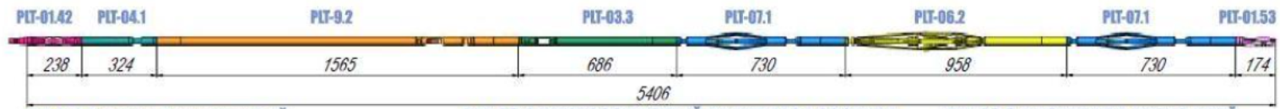
\includegraphics[width=1\textwidth]{DM/log_example.png}
\caption{Пример расположения датчиков в каротажной сборке. Здесь PLT-X - различные приборы; расстояния между ними указаны в миллиметрах.}
\label{fig:log_example}
\end{figure}

\par
Тем не менее, на первом этапе работы с полевыми данными (предоставленными нам уже после указанной предобработки) было решено проверить, насколько ситуация близка к идеальной. Корреляционный анализ показал, что рассинхронизация может превышать разумные погрешности, например 0.5м. Поэтому мы разработали и реализовали алгоритм предварительной синхронизации полевых данных. Отметим, что причинами рассинхронизации могут быть как технические сбои приборов и записывающей/считывающей аппаратуры, так и человеческий фактор. Это, вероятно, порождает ошибки в стандартных алгоритмах предобработки. Поэтому дополнительное использование корреляционного анализа позволяет распознать участки траектории с рассинхронизацией и устранить ее.
\par
В предложенном алгоритме синхронизации производится автоматическая коррекция относительных сдвигов датчиков, которые уже не обязательно будут соответствовать реальным расстояниям между ними в приборе.

\paragraph{Постановка задачи}
\par
Предположим, что имеется $N$ датчиков $\alpha_n,\;n\in[1,N]$, расположенных на некотором отрезке (сборка приборов) и генерирующих сигналы – последовательности по времени. Для удобства можно представить, что отрезок закреплен, а скважина движется относительно него. Отметим, что координата по времени однозначно пересчитывается в координату по стволу скважины через скорость движения. 
\par
Назовем вектором сдвигов набор значений $(\alpha_n,s_n),\;n\in[1,N]$, где для каждого датчика $\alpha_i,\;i\in[2,N]$ указан сдвиг $s$ показаний этого датчика относительно опорного датчика $\alpha_1$ такой, что $-10\text{м}<s_i<10\text{м}$ и $s_1=0$.
\par
В идеале все сдвиги равны нулю (датчики находятся в одной точке). В реальности они разнесены, отсюда возникает рассинхронизация последовательностей сигналов от датчиков. Нам надо найти оптимальный вектор сдвига с учетом разной физики и зашумленности сигналов. Такой сдвиг с противоположным знаком должен обеспечить синхронизацию последовательностей.

\paragraph{Алгоритм}
\par
Для разработки алгоритма анализировались данные по горизонтальной скважине Х45. На устойчивость работы алгоритма влияет много факторов, включая разную физику сигналов (температура, акустический шум, скорость флюида, фаза флюида и т.д.), зашумленность и др. Чтобы уменьшить влияние этих факторов, был выбран близкий к горизонтальному участок траектории, так как показания датчиков меньше подвержены искажениям, вызванных физической перестройкой течения в местах изменения наклона скважины. ми изменений траектории событиями. В данном случае длина участка составляла 300 метров (3000 точек). В качестве опорного датчика использовался сигнал показаний глубины – TVD (true vertical depth). 
\par
\textit{Шаг 1}. Назовем оптимальным сдвигом между двумя массивами показаний $A_1$ и $A_2$ число $s_{12}= s(A_1,A_2)$ такое, что:
\begin{equation}
    s_{12}=\arg\max_{-10\text{м}\leq s\leq10\text{м}} \left(corr(A_1,A_2-s)\right),
\end{equation}
то есть такой сдвиг, применение которого к массивам $A_1,A_2$ позволит достичь максимального коэффициента корреляции Пирсона между ними.
\par
Оптимальный сдвиг можно оценить перебором возможных значений сдвигов в диапазоне $[-10\text{м},10\text{м}]$. В первом шаге алгоритма для каждой пары показаний датчиков вычисляется оптимальный сдвиг, результатом вычисления является антисимметричная матрица 1 размера $N\times N$ (рисХ). 
\par
Отсутствующие значения в ячейках матрицы 1 означают, что максимум коэффициента корреляции был достигнут на границах рассматриваемого участка $\pm10\text{м}$. Так как длина колонны обычно не превышает $10$м в длину, такие максимумы корреляции нефизичны, то есть, на рассматриваемом интервале траектории данные не имеют заметной корреляции, и алгоритм «поймал» корреляцию уже не связанных друг с другом событий.
\par
Из-за большого количества «пустых значений» в данном случае полученная матрица 1 состоит из одного столбца и одной строки – то есть необходимые взаимные сдвиги можно получить, просто взяв эти столбец или строку. Однако, такой вид матрицы не гарантируется: в общем случае может нарушаться аддитивность оптимальных взаимных сдвигов. Поэтому автоматическое определение оптимального вектора сдвигов предполагает дополнительный шаг.
\par
\textit{Шаг 2}. Если бы отсутствовали любые сдвиги между датчиками, матрица 1 состояла бы только из нулей. Будем к этому стремиться. Назовем оптимальным вектором сдвигов такой вектор сдвигов $(\alpha_n,s_n)^{opt},\;n\in[1,N]$, при применении которого к данным матрица 1 была бы минимальной по евклидовой норме, то есть:
\begin{equation}
    S^{opt}=\arg\min_{s\in[-10,10]^N}\sum_{i,j}(M_{ij})^2
\end{equation}
При вычислении нормы матрицы отсутствующие значения полагаются равными нулю.
Для оптимизации $L_2$-нормы матрицы $M$ предлагается следующий алгоритм:
\begin{itemize}
    \item[]$S^0=[0]\times N$ – изначально нулевой вектор сдвигов,
    \item[]$i=1$ – номер строки матрицы $M$,
    \item[]$k=0$ – номер итерации,
    \item[]$\varepsilon=10^{-3}$ – регулируемый критерий останова сходимости,
    \item[]$M^0=M$ – полученная на шаге 1 матрица попарных сдвигов,
    \item[]$F^0=L_2(M)=\sum_{i,j}(M_{ij})^2$ – начальное значение минимизируемой нормы матрицы.
    \item[] while $F^k>\varepsilon$:
    \begin{itemize}
        \item[]$m=\frac{1}{N}\sum_{n=1}^N M_{in}$ 
        \item[]$S_i^k=m$
        \item[]Нулевая матрица $T^k$  размера NxN заполняется следующим образом:
        $$\forall i\in[1,..,N],\;\forall j\in[1,...,i-1,i+1,...,N]\rightarrow T_{ij}^k=m,\; T_{ji}^k=-m$$
        \item[]$M^k=M^{k-1}-T^k$
        \item[]$k=k+1$
        \item[]$i=i+1$ если $i<N$, иначе $i=0$
        \item[]$F^k=L_2(M^k)$
    \end{itemize}
\end{itemize}
\par
Таким образом, на каждой итерации из соответствующей строки матрицы вычитается ее среднее; к соответствующему столбцу добавляется это среднее для сохранения антисимметричности; вычисленное среднее добавляется к изначально пустому вектору сдвигов.
\par
На рассматриваемом примере оптимизируемый функционал в результате алгоритма уменьшился с $F^0=320.5$ до $F^K=2.5\times 10^{-4}$ за $K=10$ итераций. Результаты на примере некоторых данных скважины X45 показаны на следующих рисунках: создание и преобразование матрицы сдвигов на рис.\ref{fig:shift_matrices}, предложенная схема расположения датчиков на рис.\ref{fig:shift_log} и демонстрация сдвига данных на рис.\ref{fig:shift_signals}.

\begin{figure}[H]
\centering
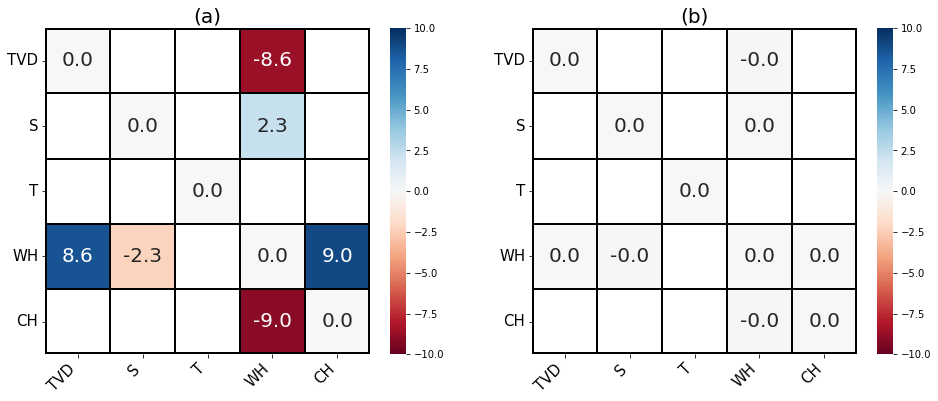
\includegraphics[width=0.8\textwidth]{DM/shift_matrices.png}
\caption{Матрицы попарных оптимальных сдвигов. (a) - вариант до оптимизации, (b) - результат после минимизации $L_2$-нормы. Видно, что удалось достичь идеального случая - с определенной точностью все несоответствия стали нулевыми.}
\label{fig:shift_matrices}
\end{figure}

\begin{figure}[H]
\centering
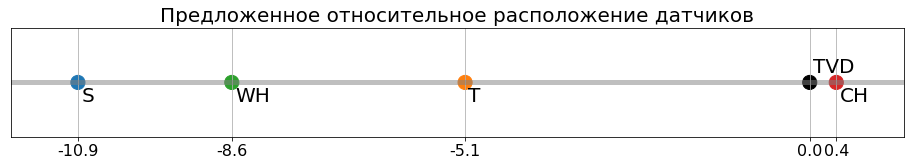
\includegraphics[width=0.8\textwidth]{DM/shift_log.png}
\caption{Примерная предложенная схема сдвига датчиков по полученным значениям. Здесь сдвиги отцентрированы относительно датчика глубины - TVD.}
\label{fig:shift_log}
\end{figure}

\begin{figure}[H]
\centering
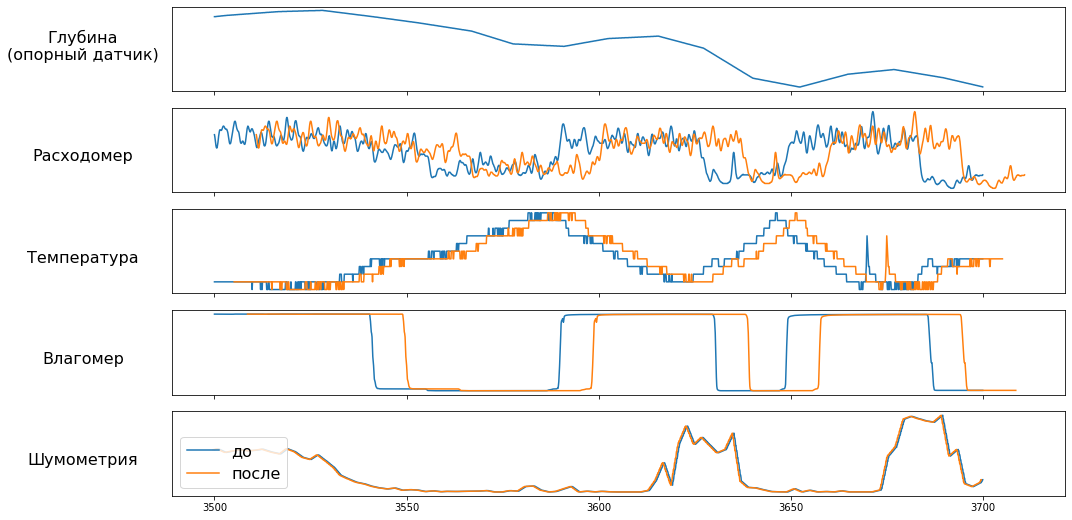
\includegraphics[width=0.9\textwidth]{DM/shift_signals.png}
\caption{Демонстрация того, как полученные сдвиги повлияли на визуальное соответствие датчиков.}
\label{fig:shift_signals}
\end{figure}

\par
Можно продемонстрировать необходимость выбора наиболее горизонтального участка траектории для анализа. На рисунках \ref{fig:shift_matrices_bad},\ref{fig:shift_log_bad},\ref{fig:shift_signals_bad} изображены матрицы получения оптимального вектора сдвигов с использованием всей траектории – порядка километра. На протяжении траектории происходит множество событий, которые вносят шум в данные. Из-за этого не получается достичь удовлетворительных результатов – оптимизация матрицы на шаге 2 мало меняет ситуацию (несмотря на то, что оптимизируемый функционал уменьшился с А до В), и применение полученных сдвигов не соответствует ранее полученным результатам и в принципе тому, что могло бы быть результатом ручной работы.

\begin{figure}[H]
\centering
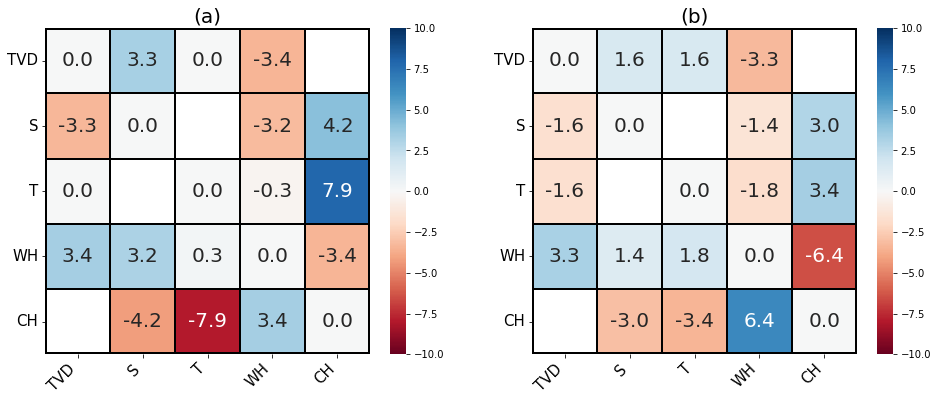
\includegraphics[width=0.8\textwidth]{DM/shift_matrices_bad.png}
\caption{Матрицы аналогично предыдущему случаю. Видно, что на втором шаге (b)  не удалось достичь идеального результата - нулевой матрицы; это показывает, что диапазон траектории для анализа был выбран неверно.}
\label{fig:shift_matrices_bad}
\end{figure}

\begin{figure}[H]
\centering
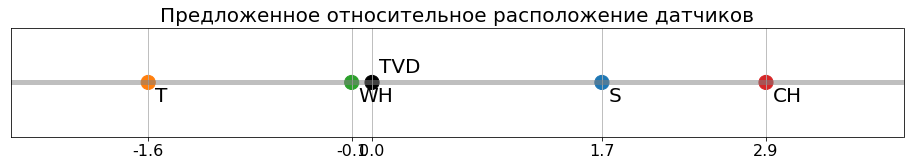
\includegraphics[width=0.8\textwidth]{DM/shift_log_bad.png}
\caption{Полученные сдвиги не совпадают с тем, что мы получили на предыдущем этапе.}
\label{fig:shift_log_bad}
\end{figure}

\begin{figure}[H]
\centering
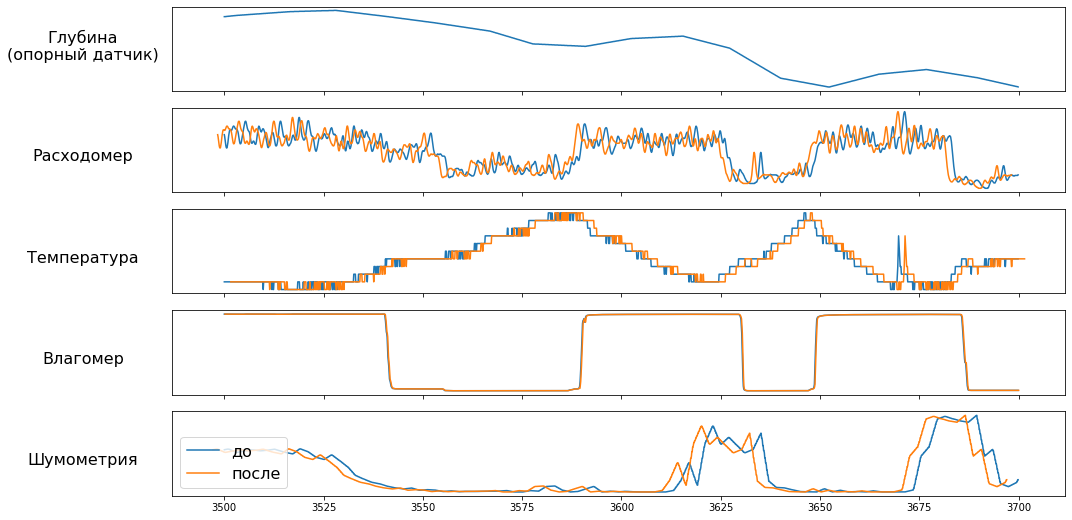
\includegraphics[width=0.9\textwidth]{DM/shift_signals_bad.png}
\caption{Видно, что алгоритм почти ничего не поменял в данных - и визуального совмещения пиков сигналов не вышло.}
\label{fig:shift_signals_bad}
\end{figure}

\subsubsection{Выделение точек изменения тренда}
\par
При анализе показаний временных последовательностей датчиков каротажной сборки приборов зачастую важны не мгновенные значения измеренных физических величин, а их тренды. Тренды могут представлять собой разрывные кусочно-линейные функции, см. пример на рис.\ref{fig:dpl_deconstruction}. Для построения таких трендов мы разработали алгоритм, основанный на распознавании точек изменения формы графика сигнала, так называемых точек «перелома» (changepoints).  
\par
Отметим, что в каротажном планшете график сигналов построен по координате вдоль ствола скважины, и его принято называть профилем. Поэтому далее в обозначениях будут использоваться сочетания «профиль» или «тренд профиля». 
\par
Построение профиля проводится нами в два этапа: вначале ищем точки перелома, затем строим профиль.
\par
Один из распространенных подходов выявления точек перелома заключается в следующем: задается некоторый функционал $\mathcal{C}$ от численного ряда, и после этого подбирается такое разбиение этого ряда, чтобы сумма значений функционалов от отрезков была меньше значения функционала $\mathcal{C}$ от всего ряда. То есть для численного ряда $y=[y_1,...,y_N]$ ищем такой набор точек $T_N={0=\tau_0<\tau_1< ...<\tau_m<\tau_{m+1}=N; m<N}$, чтобы выполнялось
\begin{equation}
    \mathcal{C}(T_N) = \sum_{i=1}^{m+1}\mathcal{C}\left(y_{\tau_{i-1}+1:\tau_i}\right)<\mathcal{C}(y)
\end{equation}
\par
Самый простой способ выбрать функцию потерь $\mathcal{C}$ – минимизировать среднеквадратичное отклонение значений ряда на отрезке.
\par
Чтобы исключить тривиальное оптимальное решение в виде разбиения всего ряда на отрезки по одной точке, вводится штраф за количество найденных разбиений, то есть минимизируется не $\mathcal{C}(T_N)$, а $\mathcal{C}(T_N)+\beta f(m)$, где $\beta$ – параметр регуляризации, $m$ – количество найденных точек перелома профиля и $f$ - обычно линейная функция $f(m)=m$.
\par
Распространенный подход оптимизации функции потерь $F=\mathcal{C}(T_N)+\beta m$ – бинарная сегментация. На каждой итерации ищется одна точка перелома, позволяющая уменьшить функцию потерь $F$. Если точка находится, каждый из двух получившихся в результате деления отрезков переходит на следующую итерацию. Алгоритм останавливается, когда значение функции потерь перестает уменьшаться. Это вычислительно эффективно, но не гарантирует оптимального деления.
\par
Для выделения оптимальных точек перелома мы будем использовать алгоритм PELT (Pruned Exact Linear Time), описанный в \cite{pelt}.
\par
Метод основан на способе оптимального разбиения, описанного в 2005 году в \cite{jackson}.
\par
Определим $F(s)$ как минимальное значение функции потерь на первых $s$ точках ряда и $T_s$ как набор $m$ точек перелома для первых $s$ точек ряда. Пусть $F(0) = -\beta$. Тогда, разворачивая определение, получаем
\begin{equation}
    \begin{split}
    F(s) =&\min_{\tau\in T_s}\sum_{i=1}^{m+1}\left[\mathcal{C}(y_{\tau_{i-1}+1:\tau_i})+\beta\right]=\\
    = &\min_{t} \left\{\min_{\tau\in T_t}\sum_{i=1}^{m}\left[\mathcal{C}(y_{\tau_{i-1}+1:\tau_i})+\beta\right]+\mathcal{C}(y_{t+1:\tau_{m+1}}+\beta)\right\} = \\
    = &\min_{t} \left\{ F(t)+\mathcal{C}(y_{t+1:\tau_{m+1}})+\beta\right\}
    \end{split}
\end{equation}

\par
Другими словами, на каждой итерации ищется оптимальное разбиение на укороченной версии ряда, после чего ряд удлиняется на одну точку и проводится проверка: осталось ли разбиение оптимальным или нужно перенести последнюю точку перелома или добавить  новую.
\par
PELT является модификацией алгоритма \cite{jackson}, позволяющей убрать некоторые точки в процессе проверки разбиения $T$ на оптимальность, чтобы ускорить вычислительный процесс. 
\par
Делается предположение, что существует такая константа $K$, что уменьшение функционала $F$ при добавлении любой точки будет как минимум больше этой константы, то есть существует минимальное гарантированное значение выигрыша от деления:
\begin{equation}
    \exists K \geq 0: \forall t < s < T \rightarrow
    \mathcal{C}(y_{t+1:s})+\mathcal{C}(y_{s+1:T})+K \leq \mathcal{C}(y_{t+1:T})
\end{equation}
\par
Предположение эмпирически доказывается в статье \cite{pelt} на примере наиболее часто используемых функций потерь $\mathcal{C}$.
\par
Таким образом, если для кандидата $t$ на новую точку разбиения выполняется условие
\begin{equation}
    F(t)+C\left(y_{t+1:s}\right)+K\geq F(s),
\end{equation}
то $t$ не является оптимальной точкой разбиения. Проверка этого условия позволяет сделать вычислительное время алгоритма линейным – отсюда название алгоритма Pruned Exact Linear Time.

\par
Показания датчиков отражают изменения различных физических величин по длине скважины. У этих физических величин есть характеристики поведения, и у датчиков есть инерция измерений – например, плавно меняющиеся показания температуры не могут отражать часто случающиеся события. Поэтому при выделении точек перелома необходимо для каждого датчика вводить свое значение параметра $P_1$ «минимальное расстояние между событиями». После задания значения $P_1$ значение штрафа $\beta$ выбирается в нашем алгоритме автоматически подбором: $\beta$ уменьшается с определенного стартового значения до тех пор, пока минимальное расстояние между всеми полученными при данном значении $\beta$ точками не станет меньше $P_1$.
Результат работы алгоритма PELT на примере сигнала расходомера с различными значениями штрафного параметра $\beta$ показаны на рис.\ref{fig:pelt}. Используется программная реализация алгоритма из библиотеки \textit{ruptures} на языке Python.

\begin{figure}[H]
\centering
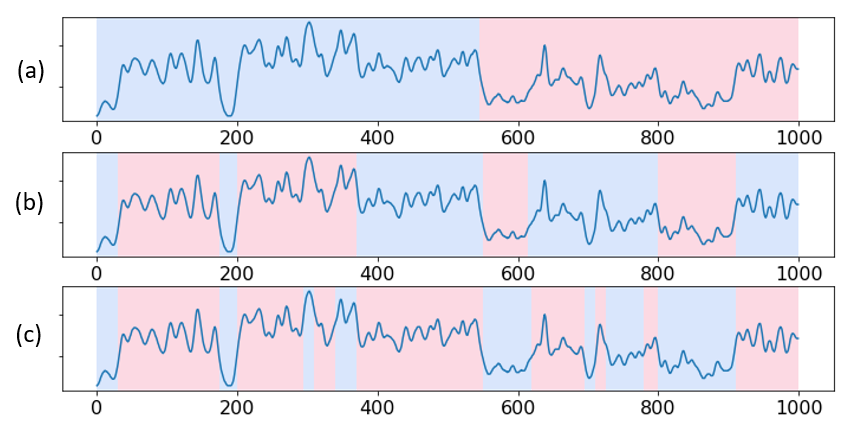
\includegraphics[width=1\textwidth]{PLT/pelt.png}
\caption{Выделенные точки перелома при различных значениях штрафного параметра $\beta: \beta_{(a)}=50, \beta_{(b)}=10, \beta_{(c)}=5$.}
\label{fig:pelt}
\end{figure}

\subsubsection{Построение разрывных трендов профиля}
\par
По полученным с помощью PELT точкам перелома теперь можно построить желаемые типы профилей. Они могут быть как разрывные (расходомер), так и непрерывные (температура). Также можно применять постоянные (влагомер), линейные (расходомер) и квадратичные функции для гладких участков профиля между точками перелома. Эти функции строятся на заданном отрезке с помощью минимизации среднеквадратичного отклонения от исходного профиля. В результате получаются различные типы профиля, которые можно обозначить как $D_n$ или $C_n$ – разрывный ($D$) или непрерывный ($C$) со степенью полинома $n=0,1,2$.
\par
Как пример рассмотрим разрывный кусочно-линейный профиль для расходомера (DPL-profile, Discontinuous Piecewise Linear profile). Желаемый результат показан на рис.\ref{fig:dpl_deconstruction}.

\begin{figure}[H]
\centering
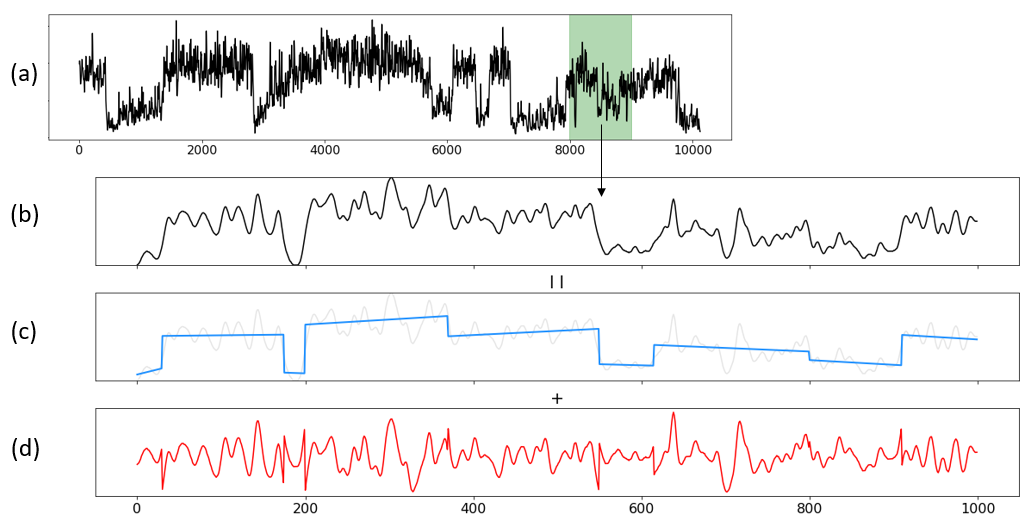
\includegraphics[width=1\textwidth]{PLT/dpl_deconstruction.png}
\caption{Пример того, как хочется преобразовать сигнал при выделении профилей. (a) - изначальный сигнал расходомера, рассматриваем выделенный зеленым участок (b). Сигнал разделяется на профиль (c) и остаточный сигнал (d), получаемый вычитанием профиля из начального сигнала.}
\label{fig:dpl_deconstruction}
\end{figure}

\par
График остатка, который характеризует «шумовую» компоненту сигнала в отличие от полезной компоненты (профиля), позволяет эксперту оценить визуально адекватность работы алгоритма.  
\par
Таким образом, нами предложена и реализована процедура построения профилей, в которой входными параметрами являются типичное минимальное расстояние между событиями (точками перелома) и тип профиля – $C_n$, $D_n$, $n=0,1,2$. Назначение этих параметров проводится экспертом – свое для каждого датчика. 

\subsubsection{Примеры результатов построения профилей}
\par
Характер поведения показаний определенного датчика предлагает вид профиля, который можно из него извлечь:
\begin{enumerate}[label=\arabic*.]
    \item Показания влагомера быстро выходят на константу, показывая различные уровни воды в точке измерения – от 0\% до 100\% . Поэтому каждый участок между двумя точками перелома аппроксимируется горизонтальным отрезком; в итоге получается ступенчатый профиль – $D_0$
    \item Показания расходомера могут как меняться плавно, так и испытывать скачки. Поэтому для каждого участка между двумя точками перелома строится линейная регрессия; в итоге получается линейный профиль с разрывами – $D_1$
    \item Показания температуры не могут испытывать скачков. Поэтому это $C_1$ или $C_2$ профили. При этом возможные небольшие разрывы в точках перелома «сшиваются». Также полезным является построение $D_1$ профилей для производной температуры, но здесь мы этот вопрос не рассматриваем.
\end{enumerate}

\par
Примеры результатов построения профилей сигналов показаны на рисунках \ref{fig:dpl_results_wh},\ref{fig:dpl_results_s},\ref{fig:dpl_results_t} на выделенных участках траектории скважины. 

\begin{figure}[H]
\centering
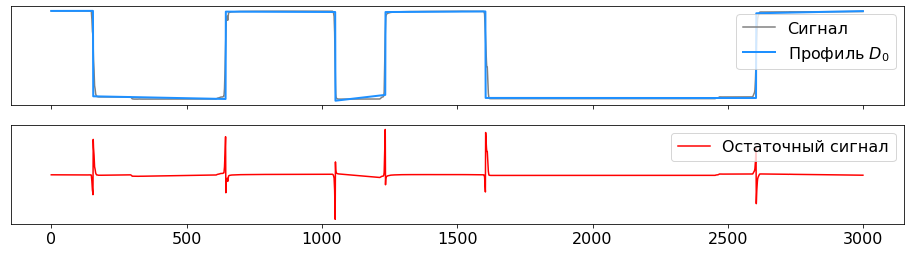
\includegraphics[width=0.9\textwidth]{PLT/dpl_results_wh.png}
\caption{Ступенчатый разрывный профиль для показаний влагомера.}
\label{fig:dpl_results_wh}
\end{figure}

\begin{figure}[H]
\centering
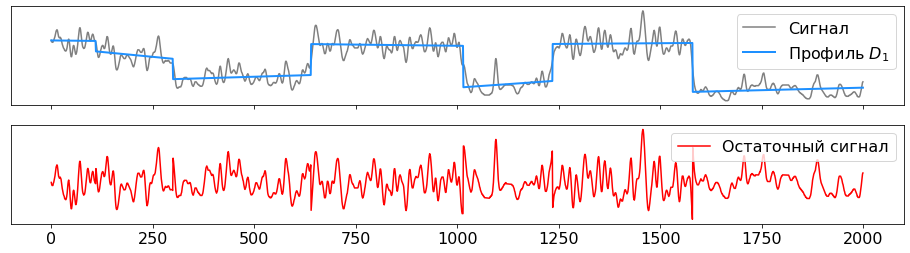
\includegraphics[width=0.9\textwidth]{PLT/dpl_results_s.png}
\caption{Кусочно-линейный разрывный профиль для показаний расходомера.}
\label{fig:dpl_results_s}
\end{figure}

\begin{figure}[H]
\centering
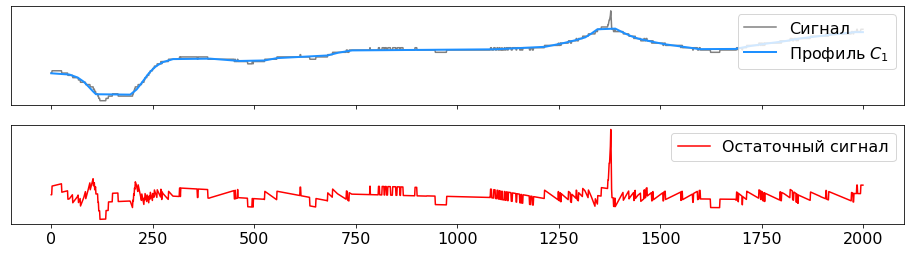
\includegraphics[width=0.9\textwidth]{PLT/dpl_results_t.png}
\caption{Кусочно-линейный профиль для показаний температуры без разрывов. В данном случае позволяет убрать ступенчатую структуру температуры, появившуюся из-за слишком маленькой вариации значений.}
\label{fig:dpl_results_t}
\end{figure}
\subsubsection{Модель слабого контроля}
\par
При построении алгоритма интерпретации на основе анализа трендов профилей, полученных в параграфе «Построение разрывных трендов профиля» для данных ПГИ и шумометрии, мы предлагаем использовать модель слабого контроля (WS, weak supervision). Это вероятностная модель машинного обучения без учителя, впервые описанная в \cite{ws} как способ быстрого создания большого количества датасетов без экспертной разметки.
\par
Суть модели заключается в объединении результатов работы слабых разметочных функций (LFs, labelling functions) в итоговую разметку. Разметочные функции – эмпирические либо любые другие правила, позволяющие решать поставленную задачу классификации – это может быть как классический вычислительный алгоритм, так и модель машинного обучения. Преимущество модели заключается в том, что разметочные функции не обязаны по отдельности быть очень точными, покрывать все множество возможных объектов для разметки или даже не противоречить друг другу; в результате обучения модель объединяет все их предсказания в одну разметку.
\par
Авторы \cite{ws} описывают WS как генеративную, или порождающую модель (generative model), то есть как вероятностную модель совместного распределения данных. Разметочные функции описываются как «шумные» - решающие задачу не полностью или неточно, и процесс обучения позволяет избавиться от этого шума, учитывая корреляции разметочных функций.
\par
Опишем вкратце процесс обучения модели на примере решения задачи бинарной классификации. Процесс обучения состоит из минимизации двух функционалов.
\par
\textit{Шаг 1.}
Назовем разметочной функцией $\lambda (x)$ функцию, которая каждому объекту обучающего датасета $S$ ставит в соответствие одну из меток {-1, 0, 1}, где метки -1 и 1 соответствуют двум классам решаемой задачи бинарной классификации, а метка 0 соответствует случаю «недостаточно информации, чтобы принять решение».
\par
Для каждой разметочной функции $\lambda (x)$ введем скалярные вероятности $\alpha, \beta$ как:
\begin{itemize}
    \item[] $\alpha$ - вероятность того, что разметочная функция разметит объект не нулем,
    \item[] $\beta$ - вероятность того, что разметочная функция разметит объект меткой -1 или 1 правильным образом.
\end{itemize}
\par
Разметочные функции порождают разметку $\Lambda$.
\par
На первом шаге подбираются параметры $(\hat{\alpha}, \hat{\beta})$ такие, что
\begin{equation}
    \hat{\alpha},\;\hat{\beta} = \arg\max_{\alpha,\beta}\sum_{x\in S}log\mathbb{P}_{(\Lambda, Y)\sim\mu_{\hat{\alpha}, \hat{\beta}}}\left(\Lambda=\lambda (x)\right)=
    \arg\max_{\alpha,\beta}\sum_{x\in S}log\left(  \sum_{y'\in\{-1,1\}} \mu_{\alpha,\beta} (\lambda(x),y')\right)
\end{equation}
\par
Другими словами, полученные оптимизацией функционала векторы параметров $(\hat{\alpha}, \hat{\beta})$ максимизируют правдоподобие полученной разметки.
\par
Здесь $\mu_{\hat{\alpha}, \hat{\beta}}$ - генеративная модель, позволяющая создавать разметку $Y$ для решения задачи бинарной классификации, используя вероятностные метки $\Lambda$ для классов {-1, 0, 1}.
\par
\textit{Шаг 2.}
После нахождения наиболее хорошо описывающих обучающий датасет наборов коэффициентов $(\hat{\alpha}, \hat{\beta})$ решается задача логистической регрессии с модифицированной лосс-функцией. Подбирается набор весов $\hat{w}$ такой, что
\begin{equation}
    \hat{w} = \arg\min_w L_{\hat{\alpha},\hat{\beta}}\left(w,S\right),
\end{equation}
где
\begin{equation}
    L_{\hat{\alpha},\hat{\beta}}\left(w,S\right) = 
    \frac{1}{|S|}\sum_{x\in S}\mathbb{E}_{(\Lambda, Y)\sim\mu_{\hat{\alpha}, \hat{\beta}}}
    \left[log\left(1+e^{-w^Tf(x)Y}\right)|\Lambda=\lambda(x)\right]
    +\rho ||w||^2
\end{equation}

\par
В этой формуле:
\begin{itemize}
    \item Логарифм под матожиданием – лосс-функция для классической задачи логистической регрессии для случая бинарной классификации с метками {-1, 1}:
    \begin{equation}
    L(Y, w^Tf(x)) = log\left(1+e^{-w^Tf(x)Y}\right)
    \end{equation}
    \item Слагаемое $\rho||w||^2$ – стандартная регуляризация весов.
\end{itemize}
\par
Поскольку разные комбинации функций разметки дают разметку разного качества, функцию потерь логистической регрессии следует скорректировать, чтобы давать более шумной разметке меньший вес. Эта коррекция выполняется с помощью функции $\mathbb{E}_{(\Lambda, Y)\sim\mu_{\hat{\alpha}, \hat{\beta}}}$.
\par
Другими словами, уровень доверия к каждой разметочной функции характеризуется коэффициентами вероятностной модели, которые подбираются в процессе обучения. Можно предложить аналогию, в которой каждая разметочная функция – это «эксперт». «Эксперты» обладают различной квалификацией: могут с различной частотой отвечать на любой вопрос «не знаю» (метка 0) и с различной частотой выдавать положительные (метка 1) и отрицательные (метка -1) ответы. Эти частоты соответствуют вероятностям $(\hat{\alpha}, \hat{\beta})$, введенным в предыдущем параграфе. Модель слабого контроля собирает всех «экспертов» в одном месте и для каждого объекта в датасете задает им вопрос – «что думаете?», а после получения меток от каждого «эксперта» на каждый объект принимает решение с учетом того, как показания «экспертов» соотносились между собой.
\par
В данной работе предлагается взять модель слабого контроля как основу для создания модели-советника – автоматизированного алгоритма интерпретации, предлагающего эксперту варианты интерпретаций для выработки окончательного заключения. Предполагается, что функции разметки могут содержать выжимку из экспертных знаний, широко описанных в литературе, чтобы экспертам не пришлось выполнять рутинную работу. Так как итоговое решение строится с оценкой неопределенности, не требуется жесткого контроля над качеством функций разметки – они должны быть просто достаточно адекватны с точки зрения специалистов.
При построении и реализации алгоритма используются программные модули  рассмотренной модели из библиотеки \textit{snorkel} на языке Python.

\subsection{Результаты}
\subsubsection{Поиск событийных участков}
\paragraph{Постановка задачи}
Рассматриваются данные горизонтальной скважины X45: датчики глубины, расходомера, температуры, влагомера и два канала пассивной акустической шумометрии – низкочастотный (0-2кГц) и высокочастотный (3-32кГц). Имеется порядка 10000 точек, записанных с шагом 0.1м по глубине скважины.
Ставится задача по имеющимся данным автоматически локализовать «событийные» участки – то есть те, на которых наблюдается отклик нескольких датчиков одновременно, что может указывать на наличие зоны притока или другие события в скважине.

Используемые для анализа данные показаны на планшете на рис.\ref{fig:data}.

\begin{figure}[H]
\centering
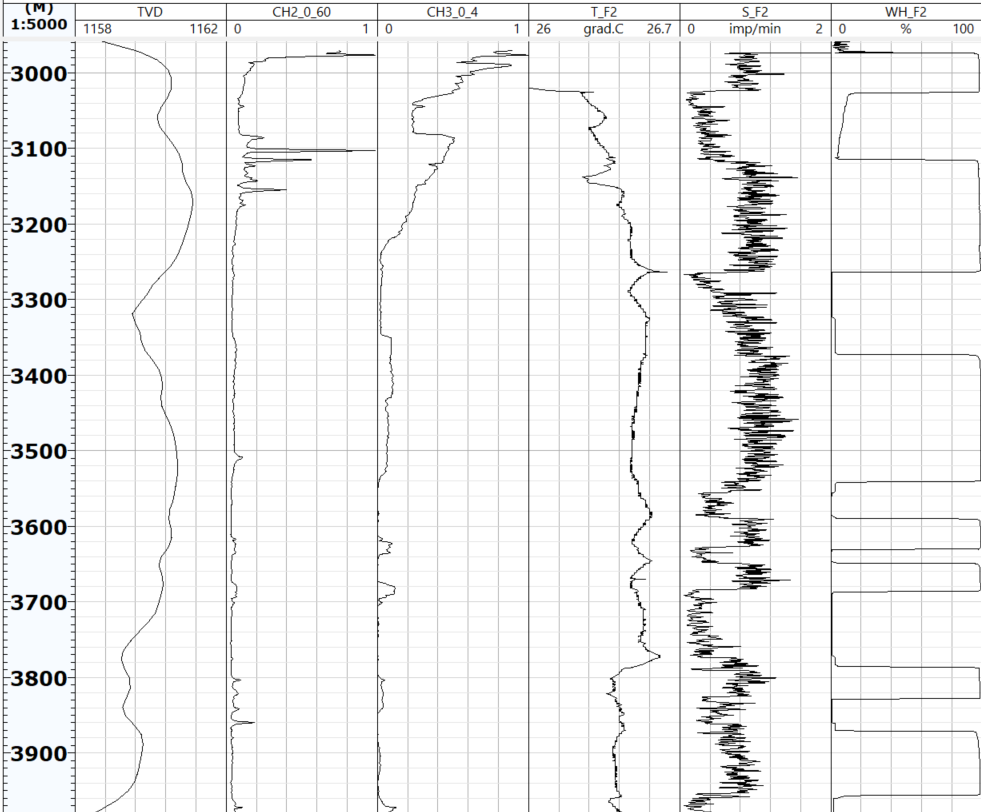
\includegraphics[width=1.0\textwidth]{WS/data.png}
\caption{Данные скважины 0X, используемые для анализа. Слева направо: показания глубины скважины, высокочастотной шумометрии, низкочастотной шумометрии, температуры, расходометрии и влагомера.}
\label{fig:data}
\end{figure}

\paragraph{Методы}
\par
Нужно локализовать отклики во всех доступных сигналах, а затем совместить их в одну разметку. Отклики могут быть несогласованы между собой различными способами:
\begin{itemize}
    \item В какой-то точке траектории есть отклики всех датчиков, кроме одного – например, в этой точке событие было, но слабое, и одному датчику не хватило чувствительности
    \item В какой-то точке траектории нет никаких откликов, кроме отклика одного датчика – например, в этой точке нет никакого значимого события, но один датчик чересчур чувствительный, и показания изменились «на пустом месте»
    \item В какой-то точке траектории часть датчиков показала отклик, а часть «промолчала» – и на первый взгляд нет однозначного решения по поводу того, каким показаниям стоит доверять.
\end{itemize}
\par
Для решения задачи, усложненной такими обстоятельствами, подойдет модель слабого контроля, описанная выше. 
\par
В выбранной терминологии, для каждого датчика можно подобрать одну или больше функций разметки – то есть экспертных правил, которые позволяют предположить, произошло на данном участке какое-то событие или нет. Функция разметки в данной постановке задачи должна выдавать один из трех ответов на каждый интервал траектории: «есть событие» (метка 1), «нет события» (метка -1), «недостаточно информации для принятия решений» (метка 0). 
\par
Здесь используем по одной функции разметки на каждый датчик. Поскольку тренды профилей для разных датчиков могут иметь разные координаты точек перелома для одного и того же события (да и событие имеет некоторую протяженность), вводится некоторое окно, которому эта метка присваивается. В данном случае окно имеет размер в 50 точек (5м). Т.е., «непрерывная» траектория при разметке заменяется на интервалы с метками через каждые 5 метров.
\par
В качестве индикатора события для расходомера, влагомера, показаний температуры и шумометрии хорошо подходят характеристики кусочно-разрывных профилей, описанных в предыдущей главе. Перед вычислением меток из всех сигналов – расходомера, влагомера, показаний датчика температуры и двух каналов шумометрии – выделяются кусочно-разрывные профили. Таким образом, для каждого сигнала у нас есть набор точек перелома, значения профиля и остаточного сигнала.
\par
Получается:
\begin{itemize}
    \item Для расходомера: считаем, что произошло событие (метка 1), если в окне находится хотя бы одна точка перелома; иначе – метка 0
    \item Для влагомера: метка 1, если в окне находится хотя бы одна точка перелома, иначе – метка 0
    \item Для температуры: метка 1, если в окне находится хотя бы одна точка, модуль значения остаточного сигнала превышает заданное значение, иначе – метка 0. Так как сигнал ввиду низкой вариативности значений практически ступенчатый, перед выделением точек перелома он был аппроксимирован сплайнами третьей степени.
    \item Для низкочастотного шума: метка 1, если в окне находится хотя бы одна точка перелома, иначе – метка 0
    \item Для высокочастотного шума: метка 1, если в окне находится хотя бы одна точка, модуль значения остаточного сигнала превышает заданное значение, иначе – метка 0.
\end{itemize}
	
\par
Указанные функции выдают только положительные либо нейтральные метки. С другой стороны, показания датчика глубины позволяют присвоить некоторым точкам отрицательные метки – то есть увеличить вероятность того, что данная точка не содержит интересующего нас события. Некоторые изменения показаний датчиков могут являться исключительно следствием влияния траектории – например, вода может накапливаться на вогнутых по отношению к горизонту участках траектории, что вызовет скачок влагомера, который нас не интересует. Поэтому вводится еще одна функция разметки:
\begin{itemize}
    \item Для траектории: метка -1, если внутри окна максимальное отклонение значений траектории от среднего значения внутри окна превышает $1.5 \sigma$ стандартных отклонений значений траектории по всей глубине скважины (внутри данного окна наблюдается большая, чем в среднем, осцилляция значений), иначе 0.
\end{itemize}
\par
Мы реализовали эту процедуру для траектории, но требуются дальнейшие исследования по повышению надежности такой разметки, поэтому здесь эти результаты не приводятся. 

\paragraph{Результаты}

На рисунках \ref{fig:lfs_signals} и \ref{fig:lfs_dpls} представлены предложенные функции разметки и результат обучения модели. Результаты работы разметочных функций – по одной на каждый датчик – пронумерованы как $\lambda_1, ..., \lambda_5$ и расположены справа от соответствующих датчиков. На рис.\ref{fig:lfs_signals} серым изображены изначальные сигналы; на рис.\ref{fig:lfs_dpls} – извлеченные из них профили для анализа.

\begin{figure}[H]
\centering
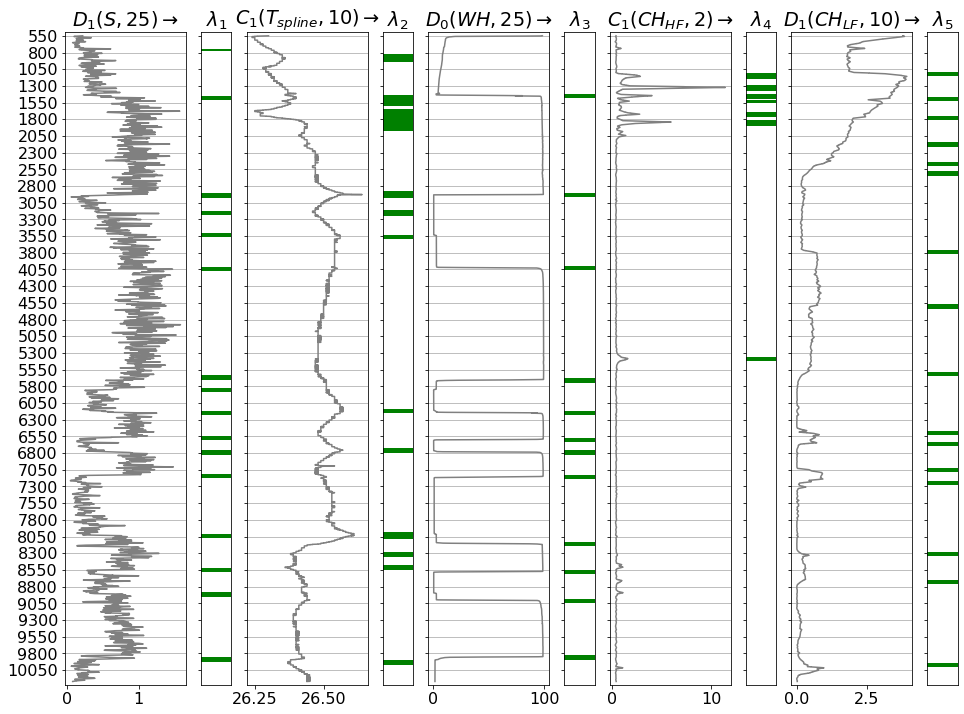
\includegraphics[width=0.8\textwidth]{WS/lfs_signals.png}
\caption{Разметочные функции, используемые для создания итоговой разметки. Серым показаны сигналы, на основе которых построены разметочные функции, зеленым выделены диапазоны, где соответствующие разметочные функции отметили вероятность события.}
\label{fig:lfs_signals}
\end{figure}

\begin{figure}[H]
\centering
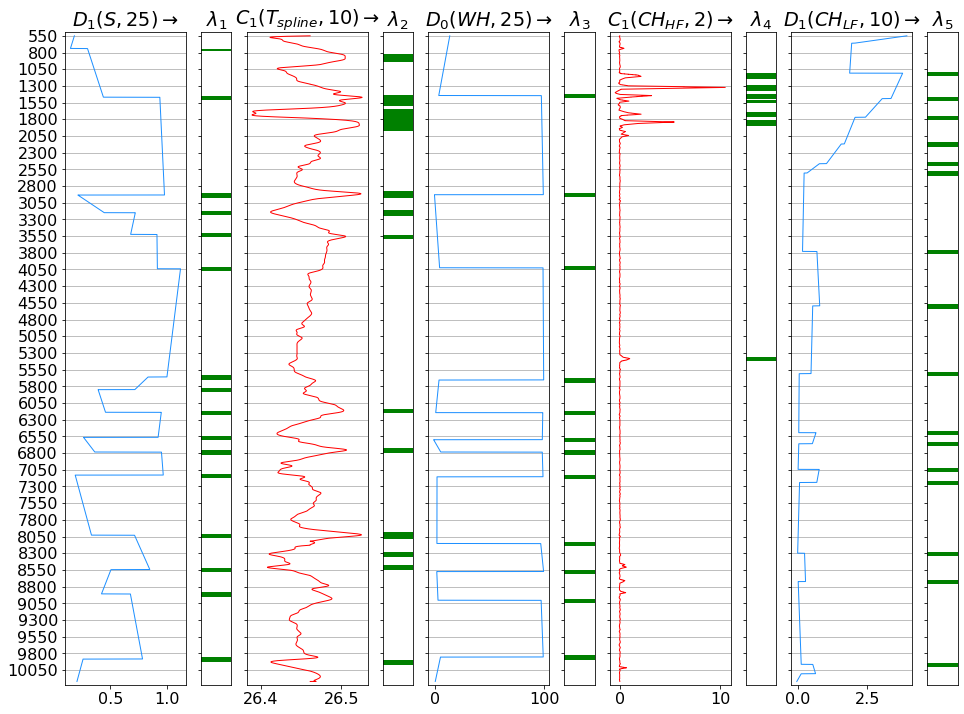
\includegraphics[width=0.8\textwidth]{WS/lfs_dpls.png}
\caption{Разметочные функции совпадают с указанными на предыдущем рисунке, но для демонстрации вместо оригинальных сигналов нарисованы выделенные профили (голубой цвет) или остаточные сигналы (красный цвет).}
\label{fig:lfs_dpls}
\end{figure}

\par
Результат работы модели – вероятностная разметка на два класса $P_{WS}$, которую можно преобразовать в дискретную разметку на два класса (1 или 0) или оставить так для оценки неопределенности. 
\par
На рисунках \ref{fig:results_optimal}, \ref{fig:results_narrow} и \ref{fig:results_wide} показаны результаты работы модели при различных параметрах минимального расстояния между событиями (значения указаны в скобках в метрах; точки разнесены на расстояние 0.1м). Первый результат предлагается считать оптимальным, следующие два получены при вариации минимального расстояния между событиями с уменьшением (\ref{fig:results_narrow}) и увеличением (\ref{fig:results_wide}) всех значений. Видно, что от этого функции разметки становятся более или менее шумными – срабатывает детекция ложных событий или наоборот, важные события оказываются пропущены. Тем не менее, общий вид итоговой разметки примерно сохраняется. Это объясняется тем, что показания температуры и высокочастотной шумометрии анализируются по значениям остатка после выделения профиля, а расходомера, влагомера и низкочастотной шумометрии – по выделенным точкам перелома. Таким образом, при увеличении минимального интервала между событиями уменьшается количество точек перелома, но становятся более шумными остатки; и наоборот – при уменьшении минимального интервала между событиями количество точек перелома увеличивается, но остатки температуры и высокочастотной шумометрии показывают меньше информации. 
\par
На рисунках \ref{fig:results_optimal}, \ref{fig:results_narrow} и \ref{fig:results_wide} класс 0 («недостаточно информации») изображен белым цветом, класс 1 («вероятно событие») - зеленым.


\begin{figure}[H]
\centering
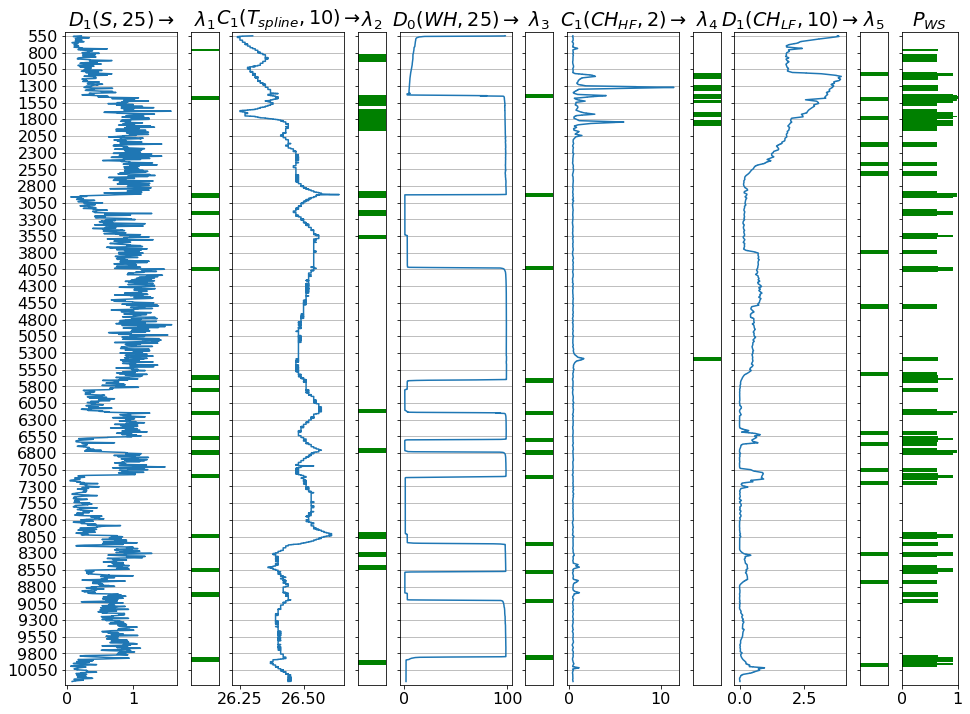
\includegraphics[width=1.0\textwidth]{WS/results_optimal.png}
\caption{Из разметочных функций в результате работы модели слабого контроля создается финальная разметка в последней колонке. Длина столбиков отражает вероятность события в данной точке.}
\label{fig:results_optimal}
\end{figure}

\par
Здесь показан результат работы модели (последний столбец $P_{WS}$) для участка в 1500 точек в приближении. 

\begin{figure}[H]
\centering
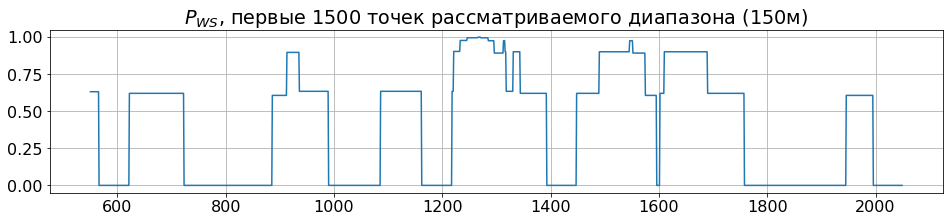
\includegraphics[width=1.0\textwidth]{WS/probability_flat.png}
\caption{Увеличенный участок последней колонки с предыдущего рисунка.}
\label{fig:probability_flat}
\end{figure}

\begin{figure}[H]
\centering
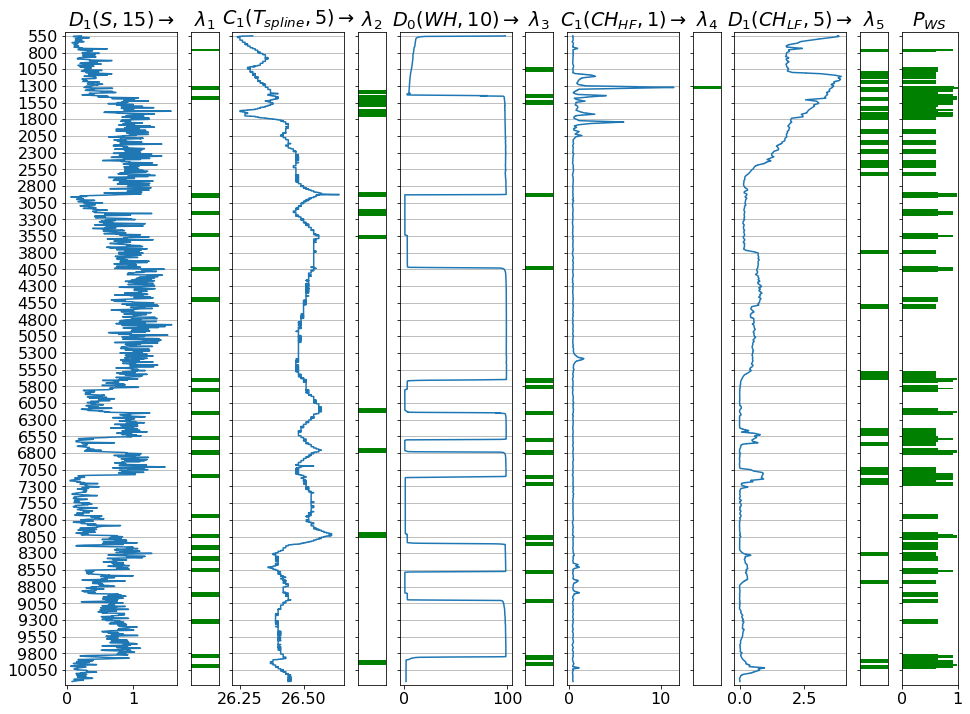
\includegraphics[width=0.8\textwidth]{WS/results_narrow.png}
\caption{Проверка устойчивости модели: для каждой разметочной функции минимальная ширина между событиями для выделения профилей была уменьшена. Видно, что финальная разметка изменилась, но не сильно.}
\label{fig:results_narrow}
\end{figure}

\begin{figure}[H]
\centering
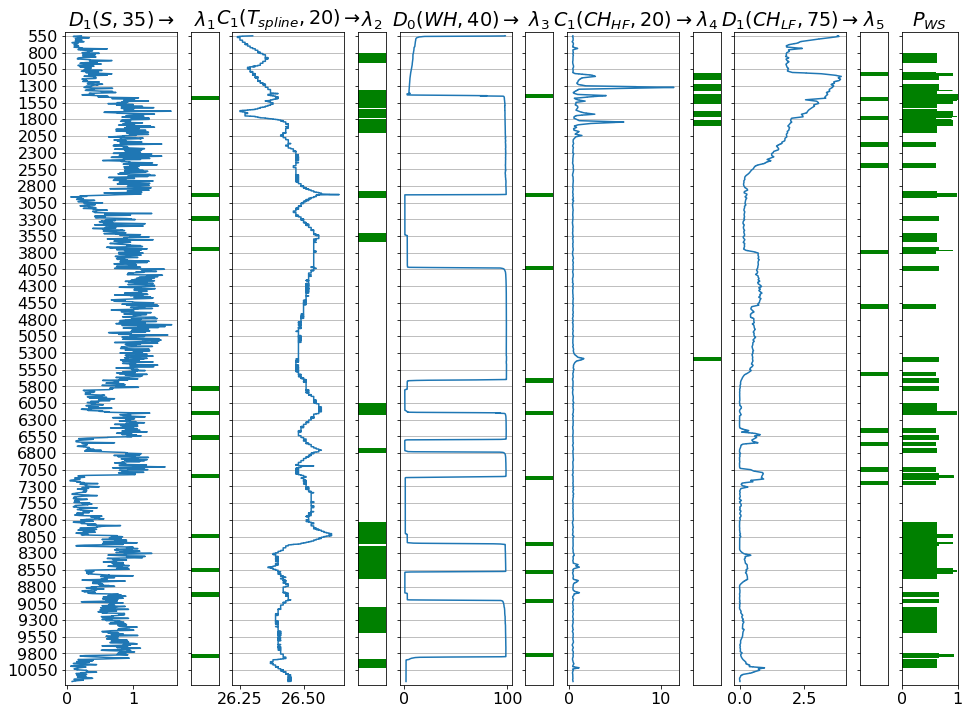
\includegraphics[width=0.8\textwidth]{WS/results_wide.png}
\caption{Аналогично предыдущему рисунку, но значения минимальной ширины между событиями были увеличены относительно оптимальных, а не уменьшены.}
\label{fig:results_wide}
\end{figure}

















\subsubsection{Детекция притока по данным температуры оптического кабеля}

\paragraph{Постановка задачи}
\par
Рассматривается вертикальная скважина L1. Для анализа доступны данные температуры, полученные с помощью волоконно-оптического кабеля, протянутого по длине скважины. Показания записывались в диапазоне порядка шести часов с шагом примерно 7 секунд – всего около 3000 измерений для участка траектории порядка 2.5км с шагом 0.5м. Пример данных в начале, в середине и в конце измерений показан на рис.\ref{fig:leakage_data}.

\begin{figure}[H]
\centering
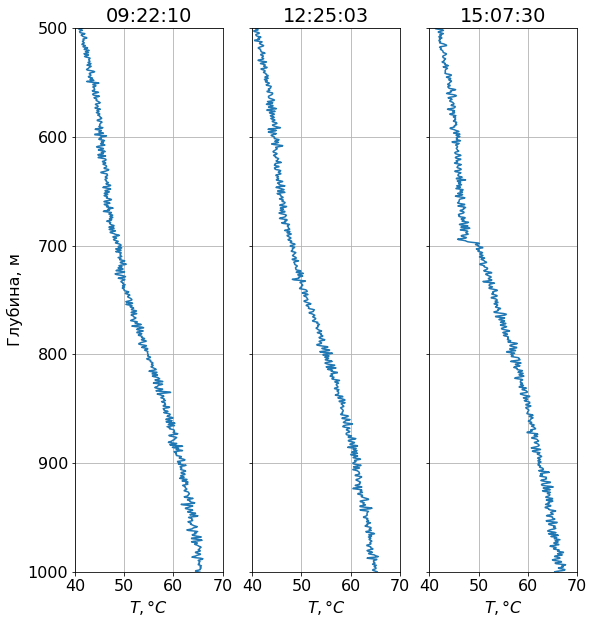
\includegraphics[width=0.8\textwidth]{PLT/leakage_data.png}
\caption{Пример данных в три различных периода времени. На третьем графике виден пик в районе 700м, на других двух он незаметен. Задача состоит в том, чтобы по всем сигналам выловить возможные пики, которые могут наблюдаться не на всем времени измерений.}
\label{fig:leakage_data}
\end{figure}

\par
Необходимо по всем доступным данным локализовать возможные места притока в скважине. Отклик от притока – температурная аномалия.

\paragraph{Методы и результаты}
\par
На предыдущем рисунке видно, что по последнему измерению можно заметить скачок температурных измерений на глубине порядка 700 м, в то время как на других двух ничего такого заметить нельзя. Данные шумные, однообразные и их много – поэтому для минимизации шума можно просто их усреднить – результат показан на рис.\ref{fig:leakage_results}(a).
\par
В полученном сигнале видно уже два скачка – на глубине порядка 700 и 1600, но они все еще слабые. Поэтому необходимо вычесть «гладкий» профиль сигнала и рассматривать только остаточный «шум». В качестве метода получения гладкого профиля выбрали кусочно-непрерывную аппроксимацию сплайнами третьей степени. После вычитания аппроксимации сплайнами остается сигнал, показанный на рис.\ref{fig:leakage_results}(b) – здесь скачки уже видны гораздо лучше.
\par
Тем не менее, в сигнале наблюдается низкочастотная осциллирующая структура, которая может быть артефактом измерений. Она автоматически убирается с помощью высокочастотного фильтра на основе преобразования Фурье (зануление в спектре всех частот ниже той, которая имеет максимальную интенсивность, и последующее восстановление сигнала). Спектр и остаточный сигнал показаны на рис.\ref{fig:leakage_results}(c),(d).
\par
Чтобы получить из данного сигнала некоторое подобие вероятности, позволяющее ранжировать только самые интересные участки, можно возвести модуль этого сигнала в какую-нибудь степень $\alpha, 1<\alpha<5$. Результат возведения в степень с $\alpha=4$ отнормирован на интервал [0,1] и показан на рис.\ref{fig:leakage_results}(e). Полученные пики для координат около 700 и 1600 локализуют места притока, а их амплитуды - «вероятность» – притока.

\begin{figure}[H]
\centering
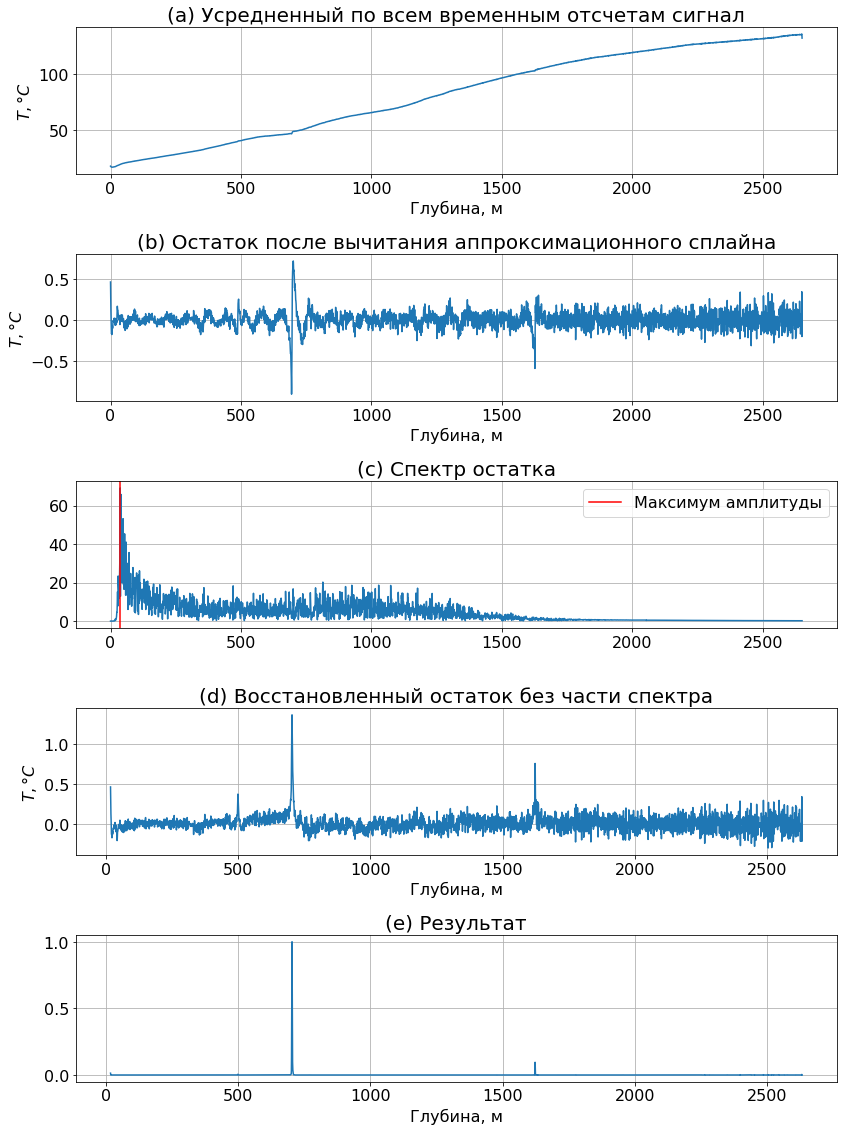
\includegraphics[width=1.0\textwidth]{PLT/leakage_results.png}
\caption{Последовательные этапы выделения полезной информации из усредненного сигнала.}
\label{fig:leakage_results}
\end{figure}
\subsubsection{Детекция и классификация зон притока на тестовой скважине}

\paragraph{Постановка задачи}
\par
В данной задаче рассматриваются данные тестовой скважины M. 
\par
Скважина имеет заранее предопределенные характеристики: в ней имеется четыре набора отверстий на известной глубине. Сверху находится клапан для входа газа, ниже – три группы отверстий для входа воды в группах по 144, 144 и 216 штук соответственно. Задача заключается в том, чтобы локализовать зоны этих перфораций и определить, какой флюид втекает – газ или вода. Схема скважины показана на рис.\ref{fig:hfnd_scheme}.

\begin{figure}[H]
\centering
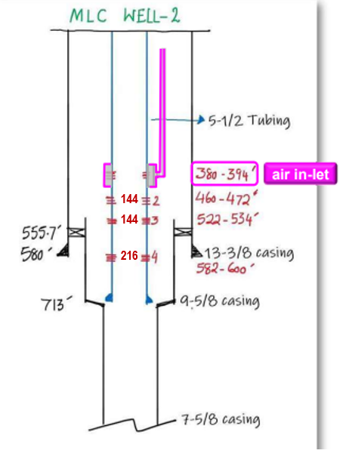
\includegraphics[width=0.5\textwidth]{PLT/hfnd_scheme.png}
\caption{Схема скважины.}
\label{fig:hfnd_scheme}
\end{figure}

\par
Для анализа используются данные прибора HFND – он содержит в себе температурный датчик и датчик пассивной акустической шумометрии. Здесь мы концентрируемся на анализе данных шумометрии. Данные записывались в диапазоне 0-100кГц с шагом 0.167м.


\paragraph{Методы и результаты}
\par
Предварительное сравнение спектрограммы со схемой перфораций показало, что отклик от притоков воды наблюдается в низких частотах, а газовый приток издает высокочастотный шум.
\par
Поэтому из всего измеряемого шумомером диапазона частот 0-100кГц для анализа мы выбрали четыре частотных диапазона:
\begin{itemize}
    \item Низкие частоты: 160-320Гц
    \item Низкие частоты, расширенные: 160-1280Гц
    \item Высокие частоты: 5-10кГц
    \item Высокие частоты, расширенные: 5-40кГц
\end{itemize}
\par
По каждому частотному диапазону в каждой точке траектории суммируются интенсивности сигналов по всем полосам, в которых производилась запись; результат показан на рис.\ref{fig:hfnd_bands}.

\begin{figure}[H]
\centering
    \subfloat[]{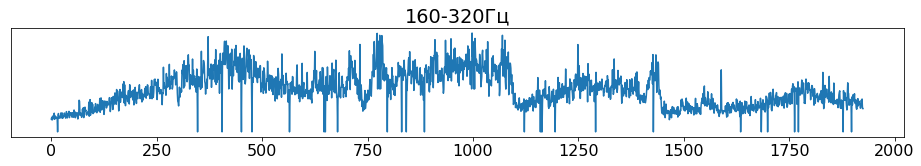
\includegraphics[width=1\textwidth]{PLT/band_1.png}}
    \vfil\vskip -20pt
    \subfloat[]{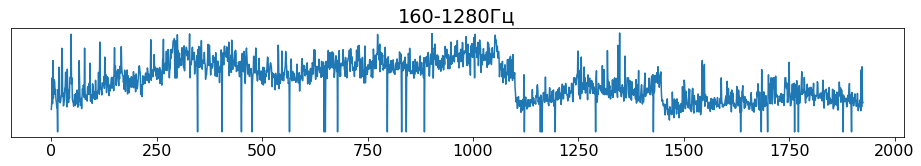
\includegraphics[width=1\textwidth]{PLT/band_2.png}}
    \vfil\vskip -20pt
    \subfloat[]{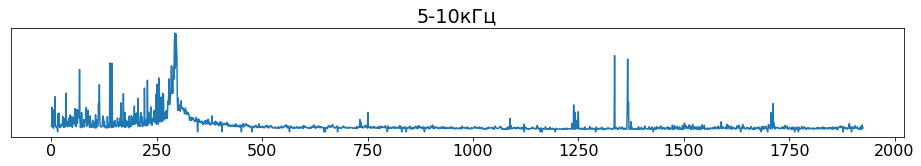
\includegraphics[width=1\textwidth]{PLT/band_3.png}}
    \vfil\vskip -20pt
    \subfloat[]{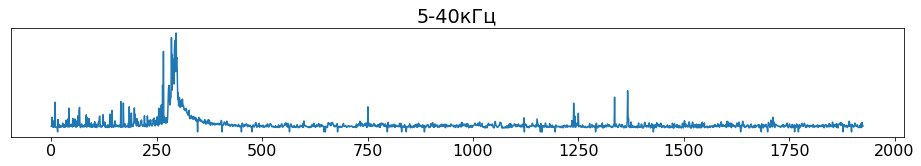
\includegraphics[width=1\textwidth]{PLT/band_4.png}}
    \vfil\vskip -20pt
\caption{Выбранные для анализа частотные диапазоны. Суммированием по всем полосам было получено усреднение интенсивности сигнала в каждой точке, которое потом используется для анализа.}
\label{fig:hfnd_bands}
\end{figure}

\par
Видно, что притоки воды можно локализовать по точкам изменения профиля интенсивности низкочастотных сигналов. Это можно объяснить следующим образом: прибор при измерении двигался снизу вверх; когда он проходил вдоль перфораций с водными притоками, притоки издавали низкочастотный шум – поэтому общая интенсивность звука увеличивалась ступенчато.
\par
Чтобы отследить это, для первых двух интервалов мы извлекаем описанные в методах разрывные кусочно-линейные профили $D_1$ и автоматически определяем участки, где скачок профиля был наибольший. Результат показан на рис.\ref{fig:hfnd_low}, скачки профиля подсвечены зеленым, искомые зоны – желтым.

\begin{figure}[H]
\centering
\subfloat[]{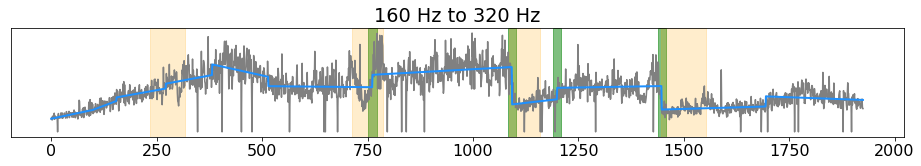
\includegraphics[width=1\textwidth]{PLT/low_1.png}}
\vfil\vskip -20pt
\subfloat[]{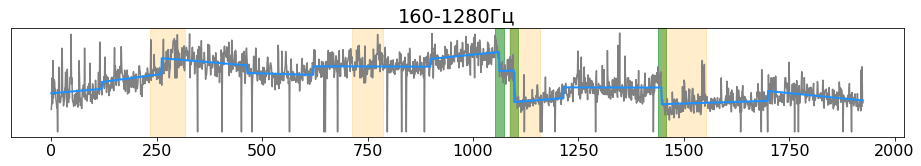
\includegraphics[width=1\textwidth]{PLT/low_2.png}}
\vfil\vskip -20pt
\caption{Результат анализа низкочастотных полос. Желтым указаны интервалы, которые хочется выделить; зеленым - полученные индикаторы. Первая полоса отвечает притоку газа, который не виден на низких частотах; другие три - водные притоки.}
\label{fig:hfnd_low}
\end{figure}

\par
Приток газа характеризуется пиком в высокочастотных диапазонах, после которого наблюдается хаотичное изменение интенсивности. Так как событие определяет пик сигнала, то мы смотрим на остаточный сигнал после выделения профиля, а не на сам профиль. 
\par
Мы хотим получить характеристику, которая служила бы индикатором хаотичности интенсивности сигнала, которая появляется после прохода зоны газового притока. Для этого сглаживаем модуль остаточного сигнала по окну и снова выделяем профиль – и ищем максимальные скачки аналогично случаю с низкими частотами. В тот момент, когда хаотичность сигнала начинает возрастать, наблюдается скачок полученной кривой. Результат показан на рис.\ref{fig:hfnd_high}.

\begin{figure}[H]
\centering
\subfloat[]{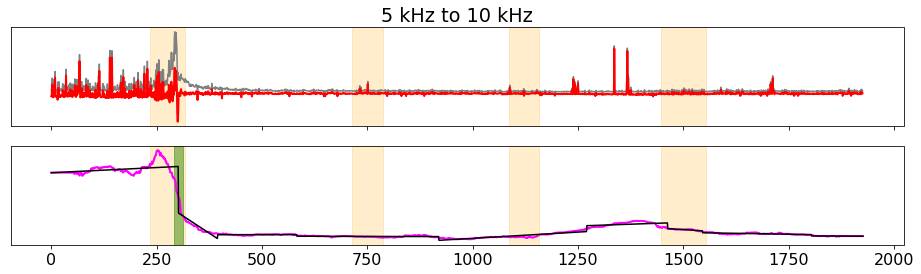
\includegraphics[width=1\textwidth]{PLT/high_1.png}}
\vfil\vskip -20pt
\subfloat[]{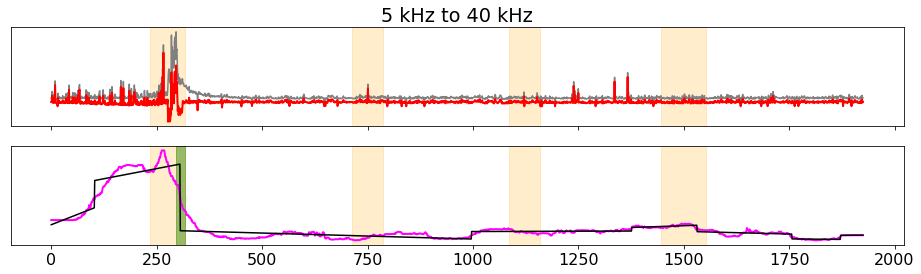
\includegraphics[width=1\textwidth]{PLT/high_2.png}}
\vfil\vskip -20pt
\caption{Результат анализа высокочастотных сигналов. Из изначального сигнала (серый) выделяется профиль и остаточный сигнал (красный). Осцилляции красного сигнала усредняются в розовый сигнал, из которого потом выделяется профиль (черный) и находится точка максимального прыжка - зеленая полоса.}
\label{fig:hfnd_high}
\end{figure}

\par
Предварительно выделенные таким образом зоны притока по низкочастотным и высокочастотным сигналам не попадают в точности в интервалы перфораций, указанные на схеме скважины. Тем не менее, их положение примерно соответствует желаемому результату; это показывает, что прибор HFND можно успешно использовать для анализа в комбинации с другими каротажными приборами.
\newpage

\section{Часть 2. Определение фазового состава флюидов вдоль ствола скважины по данным ПГИ}
\subsection{Актуальность и обоснование выбора темы}
\par
Общепринятые методы ПГИ позволяют получать высококачественные данные для вертикальных и околовертикальных скважин \cite{horizonal_1}.
\par
Специально для низкодебитных скважин в Шлюмберже разработан еще один прибор PLT-0.6.3, работа которого основана на явлении термоанемометрии \cite{horizonal_1},\cite{horizonal_2}. Интерпретация получаемых им данных проводится с целью определить фазовый состав, распределение и скорости флюидов по длине скважины. Разработаны процессы для калибровки и интерпретации данных термоанемометрии, результаты которых хорошо согласуются с результатами совместной интерпретации данных расходомера, влагомера и других ПГИ данных. Добавление PLT-0.6.3 в сборку приборов повышает качество интерпретации и увеличивает диапазон применимости сборки.
\par
Невозможность получения исчерпывающей информации о потоке флюида в скважине приводит к неоднозначности результатов интерпретации. Для построения наиболее правдоподобной интерпретации, причем с оценкой неопределенности, необходимо иметь различные варианты предсказаний фазового состава флюида на основе имеющейся информации. В данной работе предлагается дополняющий методы \cite{horizonal_1},\cite{horizonal_2} новый подход определения фазового состава флюида в скважине на основе измерений датчика термоанемометра. 
\par
Рассматривается горизонтальная газо-нефтяная скважина с наличием воды. Используемые для исследования данные получены с помощью каротажной сборки приборов, которая включает в себя базовый модуль PLT-9.2 (измеряемые величины: температура, давление, гамма-каротаж, влагомер, резистивиметр, акустический шумомер) и экспериментальный прототип распределенного термоанемометра PLT-0.6.3. Из временных рядов всех данных ПГИ для анализа мы используем данные температуры и термоанемометрии. При этом данные температуры предварительно корректируем для устранения тепловой инерции датчика.
\subsection{Описание данных}
\par
Рассматриваемый набор данных (скважина T1) содержит показания двух типов датчиков: распределенного термоанемометра – шесть одинаковых ТА датчиков, равномерно расположенных по азимуту на окружности в сечении скважины, и вспомогательного датчика, измеряющего фоновую температуру в центре окружности на оси прибора.

\subsubsection{Осевой датчик фоновой температуры}
\par
Фоновая температура в центре скважины измерена скважинным прибором PLT-9.2, который включает в себя датчик температуры со следующими характеристиками \cite{92}:

\begin{center}
\begin{tabular}{ |c|c| } 
 \hline
 Диапазон измерения температуры, $\degree C$ & от 0 до +120(150) \\ 
 \hline
 Основная погрешность измерения температуры, $\degree C$ & 1 \\ 
 \hline
 Разрешающая способность измерения температуры, $\degree C$ & 0.001 \\ 
 \hline
 Тепловая инерция измерения температуры, сек. & 1 \\
 \hline
\end{tabular}
\end{center}

\par
В исследуемом наборе данных температура записана с нерегулярно меняющимся шагом по времени от $\Delta t_{min}=0.7$ сек. до $\Delta t_{max}=4.1$ сек со средним значением $\Delta t_{avg}=1.8\pm0.6$ сек и фиксированным шагом по пространству $\Delta x=0.1$м.
\par
Разброс значений температуры лежит в интервале от $T_{min}=27.6\degree C$ до $T_{max}=28.5\degree C$ со средним значением $T_{avg}=28.3\pm0.2\degree C$.

\subsubsection{Азимутально распределенный термоанемометр}
\par
Прибор PLT-0.6.3 включает в себя шесть азимутально расположенных термоанемометров. Каждый из этих датчиков работает в цикле нагревания-охлаждения: нагревается 4 секунды и охлаждается 8 секунды. Датчики нагреваются и охлаждаются попарно – пара составляется противоположными по азимуту датчиками. Другими словами, если пронумеровать датчики по кругу номерами $i=1,..,6$, то общий циклический процесс начиная с произвольного момента времени $t=t_0$ может выглядеть так:
\begin{enumerate}[label=\arabic*.]
    \item $t_0 \leq t < t_0+4c$ : датчики 1 и 4 нагреваются; датчики 2, 3, 5, 6 охлаждаются.
    \item $t_0+4c \leq t < t_0+8c$ : датчики 2 и 5 нагреваются; датчики 1, 3, 4, 6 охлаждаются.
    \item $t_0+8c \leq t < t_0+12c$ : датчики 3 и 6 нагреваются; датчики 1, 2, 4, 5 охлаждаются.
    \item $t_0+12c \leq t < t_0+16c$ : датчики 1 и 4 нагреваются; датчики 2, 3, 5, 6 охлаждаются, 
\end{enumerate}
И так далее.
\par
Запись измерений температуры происходит каждую 0.1 секунды, что дает 120 точек на каждый цикл нагревания-охлаждения. Пример пяти последовательно измеренных циклов нагревания-охлаждения показан на рис.\ref{fig:cycle_examples}.

\newpage
\begin{figure}[H]
\centering
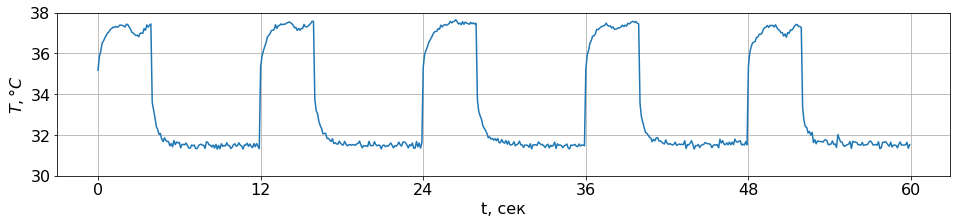
\includegraphics[width=1.0\textwidth]{TA/cycle_examples.png}
\caption{Пример пять последовательно расположенных циклов нагревания-охлаждения.}
\label{fig:cycle_examples}
\end{figure}


\subsection{Формулировка задачи}
\subsubsection{Физическая постановка задачи}
\par
Прибор движется по скважине; погруженные во флюид датчики нагреваются и охлаждаются. Характер поведения циклов нагревания-охлаждения зависит от типа флюида и его скорости относительно датчика.  
\par
Датчики термоанемометрии достаточно точные, чтобы можно было пренебречь тепловой инерцией и считать все показания измеренными с хорошей точностью; это неприменимо к осевой температуре, которая измеряется гораздо менее точным датчиком. Поэтому осевую температуру необходимо скорректировать с учетом характеристик прибора.
\par
По данным обоих приборов необходимо в общей постановке задачи определить скорость и фазовый состав протекающего через каждый датчик флюида. В данной работе опускается задача вычисления скорости флюидов, в существующих исследованиях выполняющаяся на основе корреляции признаков циклов нагревания-охлаждения с лабораторными данными. 
\par
Рассматривается задача определения фазового состава для каждого цикла. Так как скважина горизонтальная, в произвольный момент времени некоторые из шести датчиков могут находиться в разных фазах, поэтому анализ каждого датчика необходимо проводить отдельно. Отметим, что прибор может непроизвольно вращаться вокруг своей оси, продвигаясь вдоль скважины.

\subsubsection{Математическая постановка задачи}
\par
В качестве датасета рассматривается множество последовательно измеренных одним датчиком циклов нагревания-охлаждения. Под циклом понимается 120 значений температуры, измеренных с шагом 0.1 сек на некотором промежутке глубины вдоль скважины, и соответствующие этому интервалу глубины одно или несколько значений фоновой осевой температуры. Рассматривается шесть датасетов, соответствующие показаниям шести датчиков; в каждом датасете содержится около 1500 циклов.
\par
Используя доступные данные, для каждого цикла в каждом датасете необходимо предсказать метку: либо одна определенная фаза (вода, нефть, газ), либо смешанная фаза с оценкой фазового состава (например, 70\% воды и 30\% нефти).
\subsection{Используемые методы}
\subsubsection{Коррекция фоновой температуры}
\par
Для использования данных фоновой температуры необходимо учитывать два обстоятельства. Во-первых, по сравнению со временем цикла термоанемометра 12 сек температурный датчик имеет довольно значительную тепловую инерцию, равную 1 сек. (более того, мы используем только 2 сек. из 12  в предлагаемом методе анализа данных, как будет видно далее). Во-вторых, датчики термоанемометрии и измерения фоновой температуры находятся в разных приборах каротажной сборки, что приводит к возникновению естественного сдвига во временных рядах при движении этой сборки в потоке флюидов.
\par
Поэтому необходима коррекция данных фоновой температуры как по учету тепловой инерции, так и по проведению увязки по времени данных термоанемометрии и фоновой температуры.
\par
Тепловая инерция измерения температуры определяется \cite{gost} величиной показателя тепловой инерции – времени, необходимого для того, чтобы при внесении датчика в среду с постоянной температурой разность температур среды и датчика составила $e^{-1}\approx0.37$  того значения, которое будет после наступления теплового равновесия. Таким образом, за время измерения с шагом  $\Delta t=1$ сек датчик фоновой температуры $T_{bg}$ с показателем тепловой инерции 1 сек в каждой выбранной точке успевает достичь значения $\alpha(\Delta t)=0.63$ от реальной разницы между текущей и предыдущей точкой.
\par
Поскольку в исследуемом наборе данных фоновая температура записана с неравномерным шагом $\Delta t\in[\Delta t_{min},\Delta t_{max}]$, необходимо вначале построить передаточную функцию $\alpha(\Delta t)$.
Характерный вид кривой разгона термометра показан на рис.\ref{fig:thermal_inertia_curve}(а) \cite{thermal_inertia_patent}. Эту кривую приближенно можно представить как 

\begin{equation}
    T(t) = T_0 \left(1-e^{-\frac{t}{\varepsilon}}\right),
\end{equation}

где $\varepsilon$ - коэффициент тепловой инерции \cite{thermal_inertia_paper}, рис.\ref{fig:thermal_inertia_curve}(б). Так как для выбранного датчика $\varepsilon=1$с, то для рассматриваемого датчика получаем 

\begin{equation}
    \alpha(\Delta t) = 1 - e ^ {-\Delta t}
\end{equation}

\begin{figure}[H]
\centering
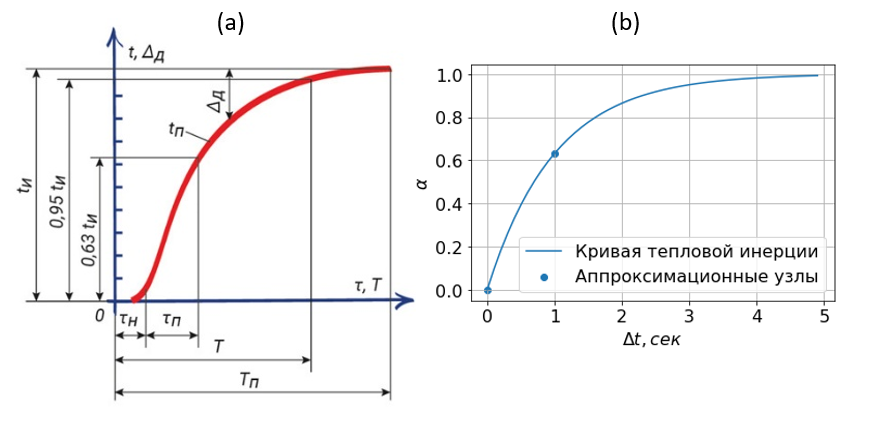
\includegraphics[width=1.0\textwidth]{TA/thermal_inertia_curve.png}
\caption{Характерный (a) и аналитический (b) виды кривой разгона термометра (передаточной функции). Для используемого датчика $\tau_H+\tau_\Pi=1$.}
\label{fig:thermal_inertia_curve}
\end{figure}

\par
Для вычисления «истинной» фоновой температуры $T_{bg}(t^i)$ обозначаем данные показаний датчика фоновой температуры через $T_d(t^i)$ и составляем следующее уравнение:
\begin{equation}
    T_{bg}(t^{i+1})-T_d(t^{i+1})=    \left(1-\alpha\right)\left(T_{bg}(t^{i+1})-T_{bg}(t^i)\right)
\end{equation}
Из него получаем формулу вычисления фоновой температуры:
\begin{equation}
    T_{bg}(t^{i+1})=T_{bg}(t^i)+\frac{T_d(t^{i+1})-T_x{bg}(t^i)}{\alpha}
\end{equation}

Результат работы алгоритма на некотором участке временного ряд для 50 точек показан на рис.\ref{fig:thermal_inertia_result}.
\begin{figure}[H]
\centering
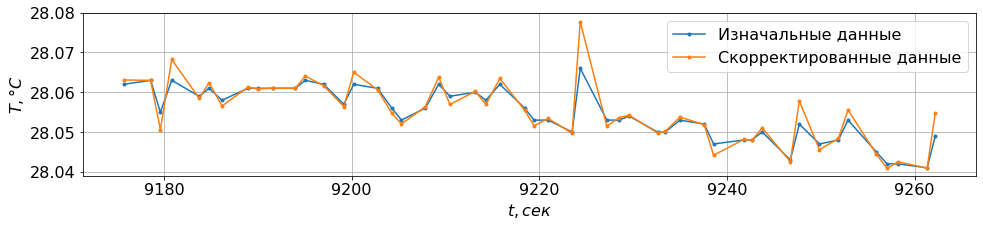
\includegraphics[width=1.0\textwidth]{TA/thermal_inertia_result.png}
\caption{Результат работы алгоритма коррекции тепловой инерции на 50 точках.}
\label{fig:thermal_inertia_result}
\end{figure}
\par
Для коррекции естественного сдвига во временных рядах данных термоанемометрии и фоновой температуры при движении сборки приборов в потоке флюидов мы вводим расстояние $L$ по стволу скважины между датчиками и относительную скорость $V$ приборов и потока. Тогда, очевидно, искомый сдвиг по времени $\delta t$ оценивается как
\begin{equation}
    \delta t = \frac{L}{V},
\end{equation}

а вычисление значений $T_{bg}(t^i-\delta t)$ проводится линейной интерполяцией.

\par
Полученные значения фоновой температуры используются для решения задачи разделения флюидов совместно с данными термоанемометра, рассматриваемой в следующем параграфе.

\subsubsection{Анализ данных распределенного термоанемометра}
\par
Рассматривается задача определения фазы флюида для каждого цикла. Экспериментальные исследования показывают, что форма циклов зависит от скорости флюида и его физических характеристик, см. рис.\ref{fig:cycle_examples_dem}.

\begin{figure}[H]
\centering
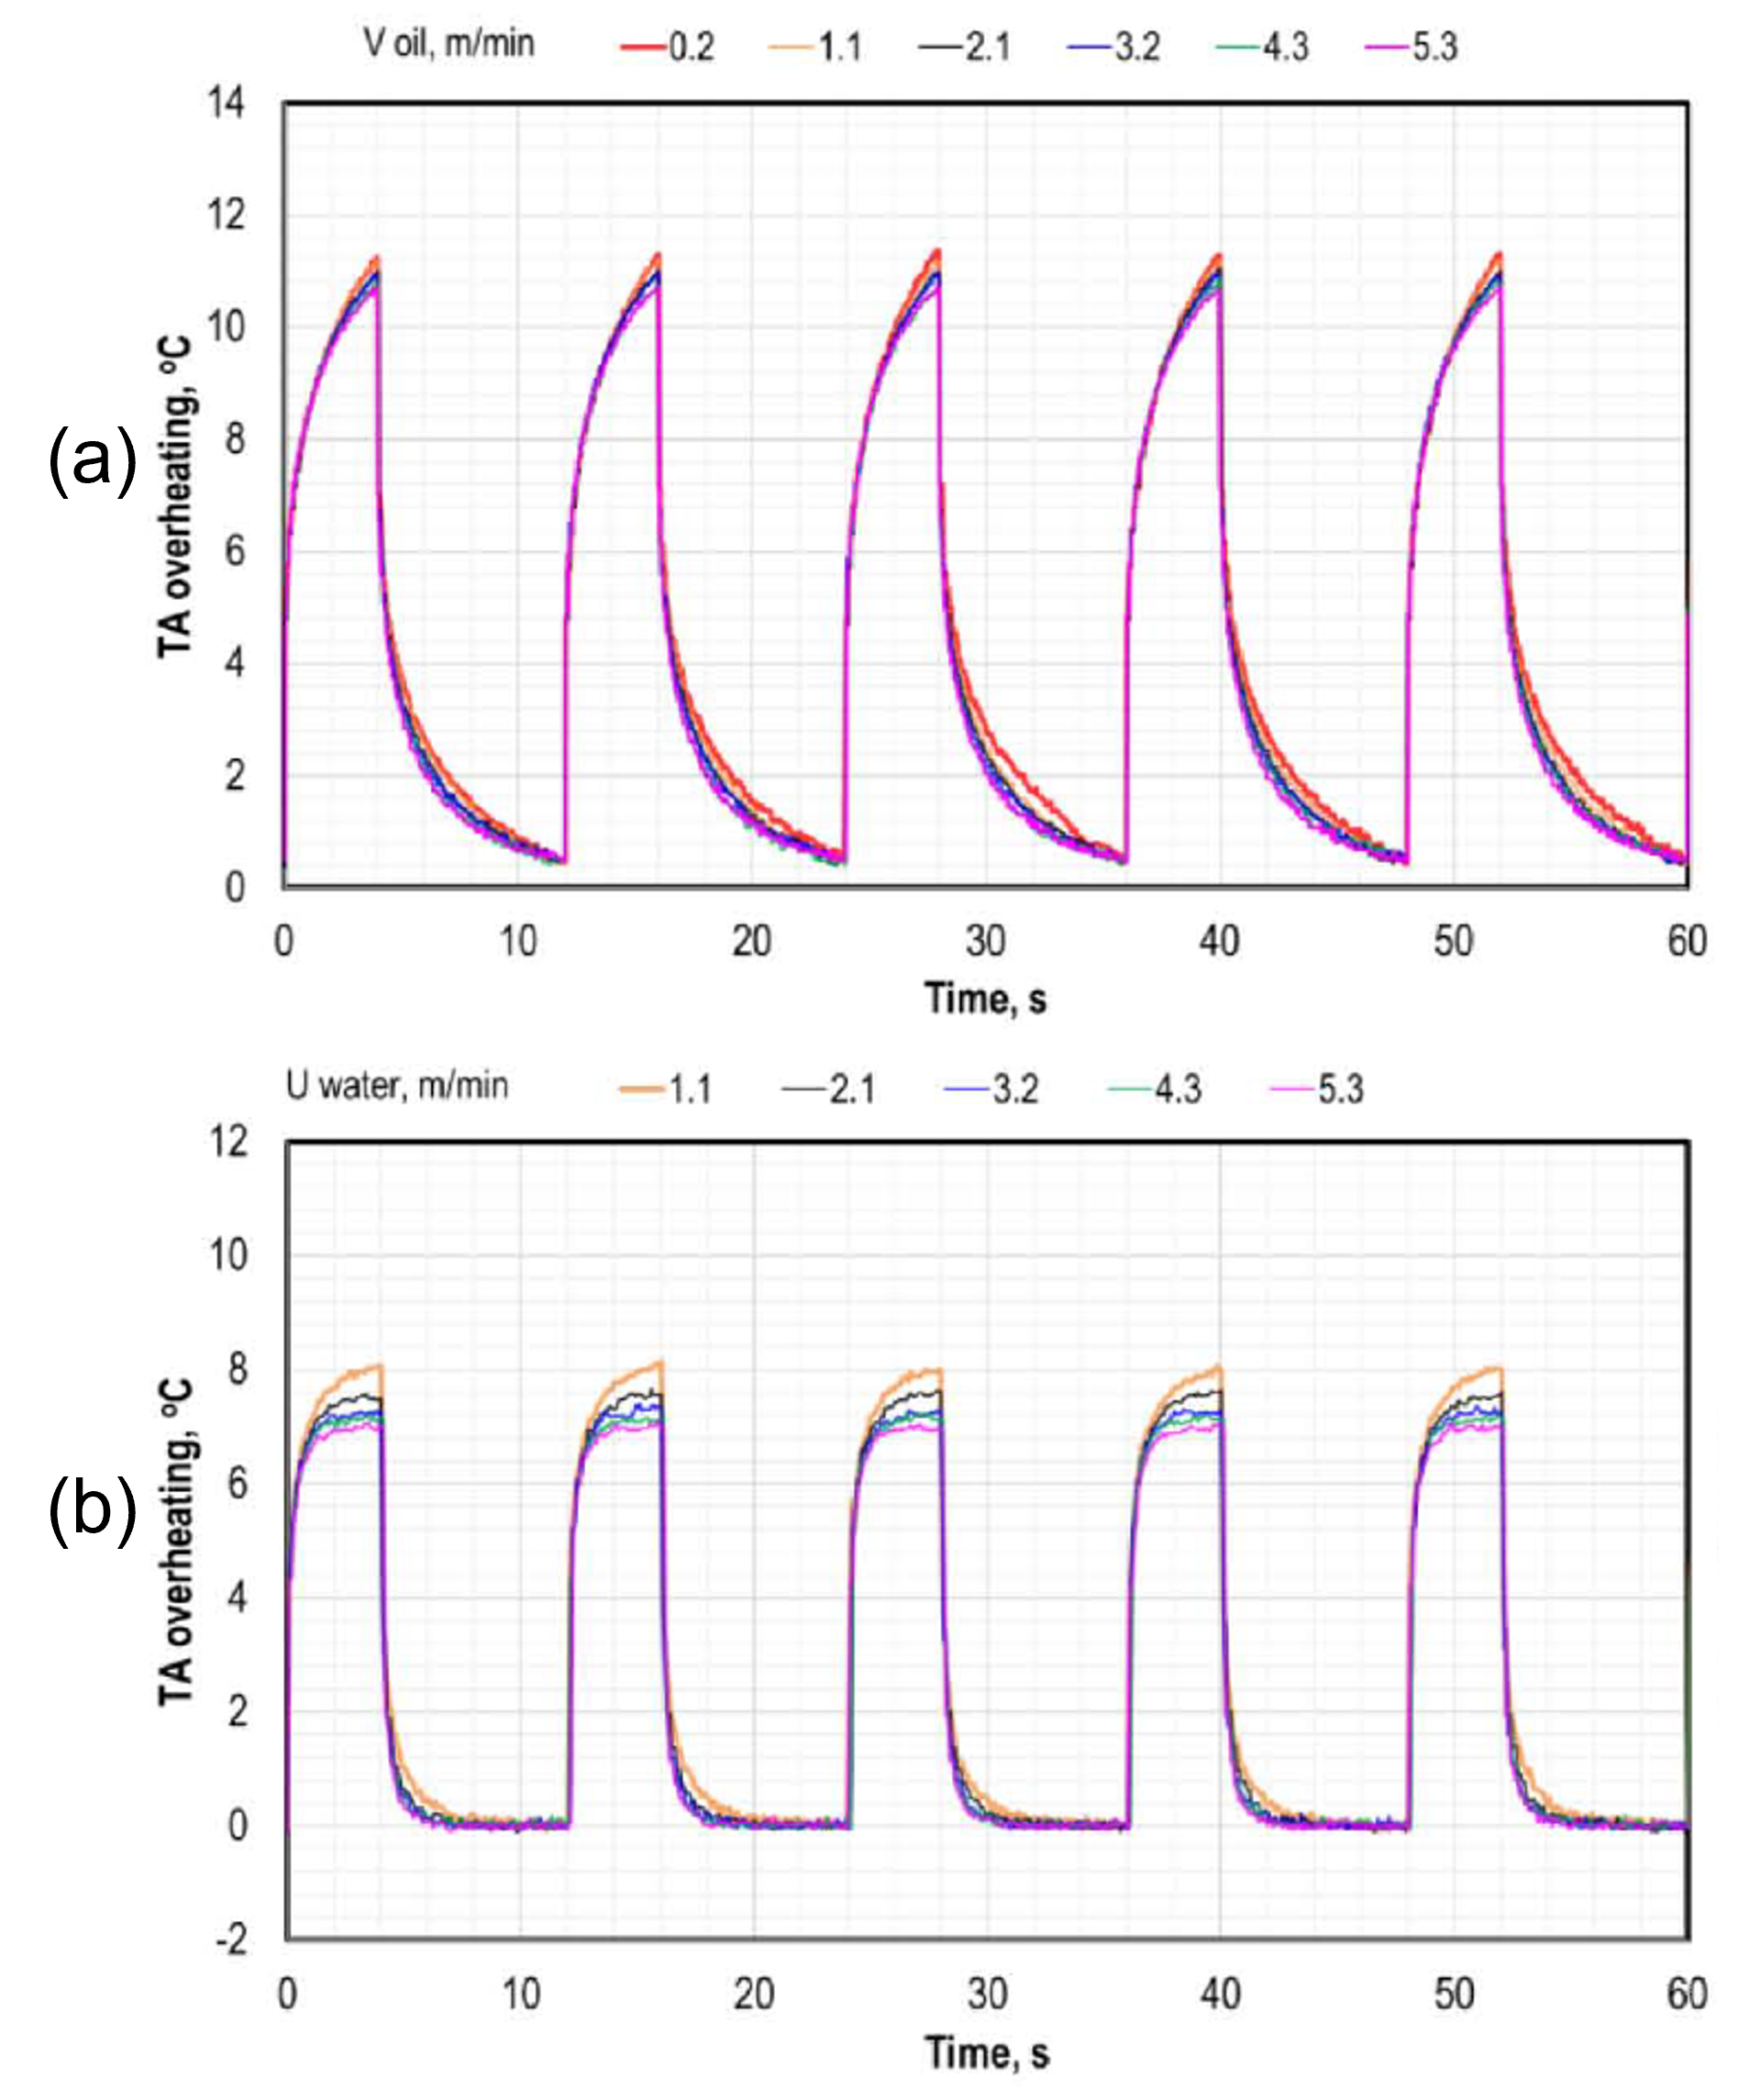
\includegraphics[width=0.6\textwidth]{TA/cycle_examples_dem.png}
\caption{Характерные циклы нагревания-охлаждения для нефти (a) и газа (b) при различных скоростях потока на протяжении пяти последовательных циклов. Лабораторные данные, результаты статьи \cite{horizonal_1}.}
\label{fig:cycle_examples_dem}
\end{figure}

\par
Изменения скорости и характеристик флюидов в определенных пределах могут вызывать изменения численных характеристик кривой графика также в определенных пределах, присущих каждому из трех типов циклов. Назовем такие численные характеристики индикаторами. Например, используются следующие индикаторы:

\begin{enumerate}
    \item[$I_1$] - разность максимальной и минимальной температур цикла
    \item[$I_2$] - производная кривой цикла в конце фазы охлаждения
    \item[$I_3$] - производная кривой цикла в конце фазы нагревания
    \item[$I_4$] - интеграл кривой цикла на протяжении фазы охлаждения
    \item[$I_5$] - интеграл кривой цикла на протяжении фазы нагревания
\end{enumerate}
и другие.
\par
На данный момент процесс интерпретации данных термоанемометрии на основе  и некоторых других (в том числе, лабораторных) измерений включен в алгоритм обработки ПГИ данных \cite{horizonal_1},\cite{horizonal_2}.
\par
Из рис.\ref{fig:cycle_examples_dem} видно, что практически все указанные индикаторы хорошо различают две фазы (нефть, вода) независимо от рассмотренных значений скорости потока. Однако, если скорости и параметры флюида претерпевают значительные изменения, то и интервалы изменений индикаторов могут пересекаться для различных фаз. Можно также отметить и другие проблемы обработки измерений, усугубляющие неоднозначность соответствия какого-либо индикатора определенной фазе, например:
\begin{itemize}
    \item Все датчики термоанемометрии немного отличаются, требуется калибровка
    \item Использование лабораторных данных требует знания характеристик флюидов и корректировки на скважинные условия
    \item Распознавание газовой фазы вызывает затруднение из-за близости значений индикаторов для нефти и газа во многих случаях
    \item За время цикла 12 сек может произойти смена фаз, что приводит к неоднозначности интерпретации индикаторов
\end{itemize}
\par
Цель исследования - уменьшение влияния указанных проблем на результаты распознавания фаз воды, нефти и газа (в идеале – исключения влияния). Важным условием является также и то, что разрабатываемый метод не должен использовать экспертную разметку данных, поскольку она недоступна в необходимом объеме, например, для алгоритмов обучения с учителем.
\par
В результате исследований поведения различных циклов из используемого датасета мы разработали метод обработки измерений, в котором подобраны индикаторы и составлены из них комбинации, т.е. признаки, позволившие использовать методы кластеризации для достаточно четкого распознавания всех трех фаз.

\paragraph{Создание признакового пространства.} 
\par
Для построения алгоритма анализировались скважинные данные примерно 1500 циклов одного из датчиков. Обозначим температуру одного цикла как $T(t_i),\;i=1,...,120$. Для упрощения обозначений мы опускаем индексы номера цикла и номера датчика из датасета и полагаем, что время соответствует абсолютному значению в датасете.  В течение интервала записи данных цикла (12 секунд) датчик может перейти из одной фазы в другую. Чтобы уменьшить вероятность влияния этого события на результат, мы используем только небольшую часть цикла для построения индикаторов, и рассматриваем точки из интервала $i=40,...,59$, т.е. 2 секунды. Это включает в себя последнюю точку фазы нагревания $i=40$ и начало фазы охлаждения. Поскольку замеры искажены случайным шумом, мы аппроксимируем точки фазы охлаждения  параболой для вычисления значений температуры и ее производной в первой точке фазы охлаждения. Обозначим эту параболу через $T^C(t)$. 
\par
После анализа, в том числе и путем перебора, в качестве индикаторов были выбраны
\begin{equation}
    T(t_{40}),\quad T^C(t_{41}),\quad \frac{dT^C}{dt}(t_{41}),\quad T_{bg}(t_{41}),
\end{equation}

где $T_{bg}$ - фоновая температура, вычисляемая согласно алгоритму из предыдущего параграфа.
\par
Чтобы уменьшить влияние скважинных условий и отличий характеристик датчиков, мы проводим обезразмеривание по температуре и формируем два признака из предложенных четырех индикаторов:

\begin{equation}
    F_1 = \frac{\frac{dT^C}{dt}(t_{41})}{T(t_{40})-T^C(t_{41})},\quad F_2 = \frac{T(t_{40})-T_{bg}(t_{41})}{T(t_{40})-T^C(t_{41})}
\end{equation}
\par
Признаки имеют простой физический смысл: $F_1$ с размерностью $\left[\frac{1}{\text{сек}}\right]$ характеризует скорость начала охлаждения, а безразмерный  $F_2$ характеризует масштаб перепада температур после окончания нагрева. Отметим, что в обезразмеривании по времени (т.е., исключении $\left[\frac{1}{\text{сек}}\right]$) нет необходимости, так как шаг по времени 0.1 сек в цикле измерений фиксирован для всех датчиков.
На рис.\ref{fig:sensor_1_raw_data}(а) в координатах $\left(F_1, F2\right)$ построены точки для измерений одного из датчиков.  Отчетливо видны три облака с приведенными условными границами (линии), которые могут соответствовать трем типам флюидов – воде, нефти и газу. Отметим достаточно изотропную форму каждого из облаков. На карте плотности точек, рис.\ref{fig:sensor_1_raw_data}(б), хорошо высвечиваются «водяной» и «нефтяной» кластеры («газовый» кластер практически не высвечивается из-за существенно меньшего количества точек в нем).

\begin{figure}[H]
\centering
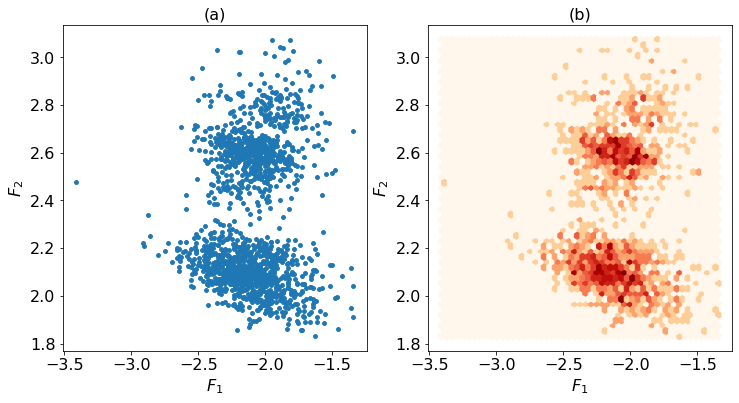
\includegraphics[width=0.8\textwidth]{TA/sensor_1_raw_data.png}
\caption{Скважинные данные термоанемометра для одного из датчиков (около 1500 точек) в координатах предложенных признаков (а) и их раскраска в соответствии с плотностью точек (б)}
\label{fig:sensor_1_raw_data}
\end{figure}

\paragraph{Кластеризация признакового пространства}
Разделение данных в полученном пространстве на три кластера делается с помощью модели смеси гауссовских распределений. Так как верхний кластер, который мы будем обозначать как «газ», содержит существенно меньше точек, и он гораздо ближе к среднему кластеру, который мы будем обозначать как «нефть», то кластеризация проводится в два этапа:
\begin{itemize}
    \item[1.] Модель 1 классификации на 2 гауссовских распределения отделяет нижний кластер («вода») от двух верхних.
    \item[2.] Оставшиеся после удаления нижнего кластера данных разделяются моделью 2 классификации на 2 гауссовских распределения на два кластера – «нефть» и «газ».
\end{itemize}

Процесс создания итоговой разметки продемонстрирован на рис.\ref{fig:sensor_1_clustering_process}. 

\begin{figure}[H]
\centering
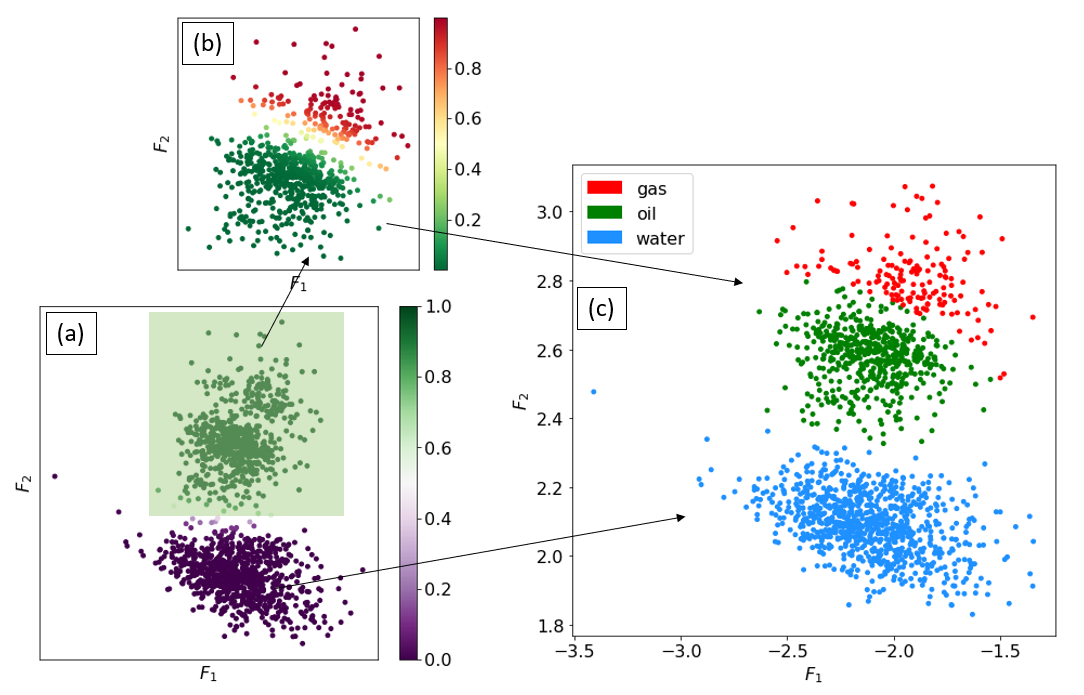
\includegraphics[width=1.0\textwidth]{TA/sensor_1_clustering_process.png}
\caption{Процесс создания итоговой разметки. Сначала (a) нижний водяной кластер отделяется от верхнего; верхний кластер разделяется (b) на нефть и газ. Полученные в результате работы двух GMM-моделей метки объединяются в итоговую (c).}
\label{fig:sensor_1_clustering_process}
\end{figure}

\paragraph{Определение положения и фазового состава точек смены фаз}
\par
Переход между фазами, то есть изменение характеристик цикла, соответствует переходу между кластерами в координатах $\left(F_1, F2\right)$. Пример перехода между фазами продемонстрирован на рис.\ref{fig:sensor_1_phase_change_demo}.  Раскраска точек соответствует полученной ранее дискретной разметке. Справа показаны восемь последовательно измеренных циклов, на основном графике стрелками тех же цветов соединяются точки в координатах $\left(F_1, F2\right)$, соответствующие этим циклам. Прибор двигался от меньшего номера цикла к большему, то есть от голубого цвета к розовому. Видно, что изменения формы циклов нагревания-охлаждения соответствуют перемещениям в выбранном пространстве признаков.

\begin{figure}[H]
\centering
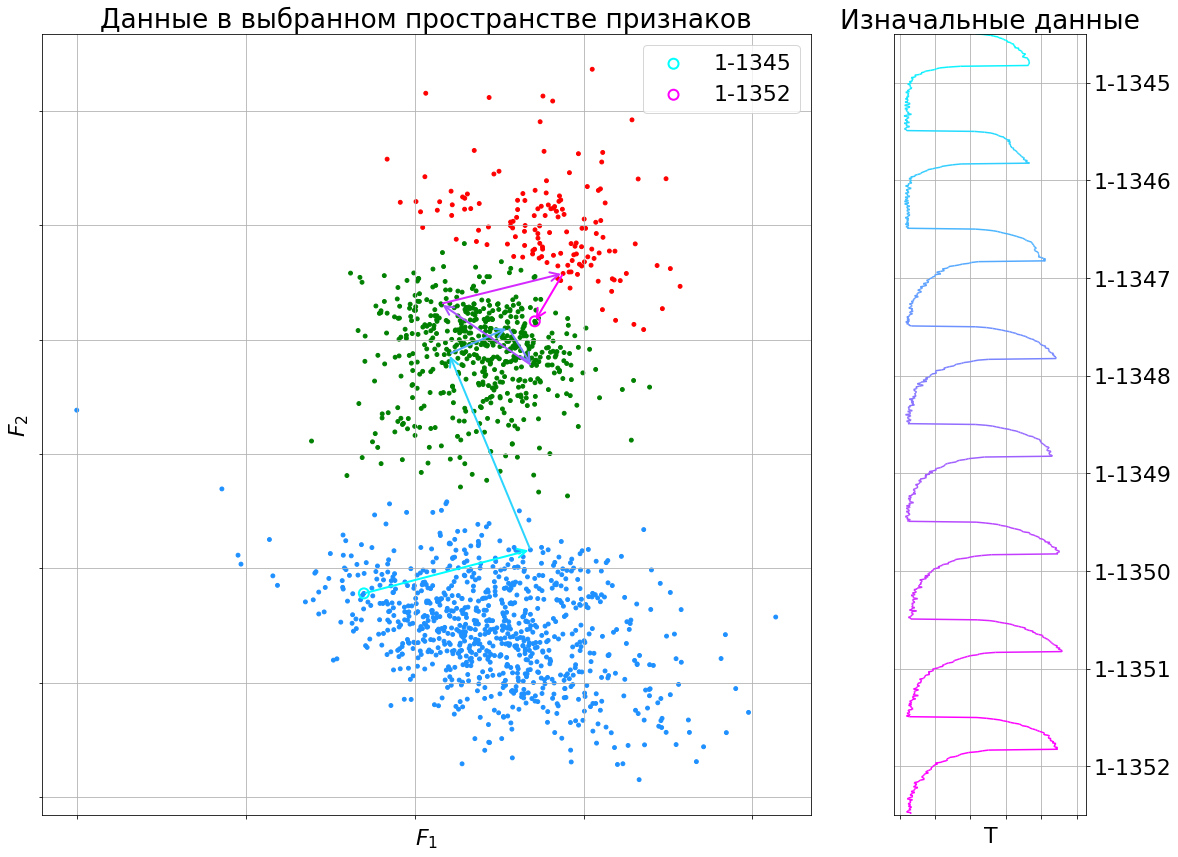
\includegraphics[width=1.0\textwidth]{TA/sensor_1_phase_change_demo.png}
\caption{Демонстрация того, как точки переходят между фазами. На правой колонке видно, как на протяжении 8 циклов меняется форма цикла - и это отражается движением точек, соответствующих этим циклам в выбранном признаковом пространстве. Движение начинается с голубого цикла, находящегося в водяном кластере, и заканчивается в розовом цикле, находящимся на границе нефтяного и газового кластера.}
\label{fig:sensor_1_phase_change_demo}
\end{figure}

\par
Необходимо автоматически определять точки смены фаз и присваивать им оценку фазового состава флюидов.
Так как разделение на кластеры производится вероятностной моделью, то дискретные метки вода-нефть-газ получаются из вероятностных оценок нахождения выбранной точки датасета в каждой из фаз. Так как разделение делается дважды: сначала отделяется вода, а потом разделяются нефть и газ, то на самом деле «сырой» результат работы модели – это два набора вероятностей.  
\par
Поэтому:
\begin{enumerate}[label=\arabic*.]
    \item Для каждой точки из класса «вода» доступны вероятности $p_{water}^1$ и $p_{oil}^1$ такие, что $p_{water}^1+p_{oil}^1=1$.
    \item Для каждой точки из класса «нефть» доступны вероятности $p_{water}^1$ и $p_{oil}^1$ такие, что $p_{water}^1+p_{oil}^1=1$; а также вероятности $p_{oil}^2$ и $p_{gas}^2$ такие, что $p_{oil}^2+p_{gas}^2=1$.
    \item Для каждой точки из класса «газ» доступны вероятности $p_{oil}^2$ и $p_{gas}^2$ такие, что $p_{oil}^2+p_{gas}^2=1$.
\end{enumerate}

\par
Форма и процесс получения выделяемых кластеров в координатах $\left(F_1, F2\right)$ предполагает только два варианта точек смены фаз: «вода-нефть» и «нефть-газ»; вариант «вода-газ» не выделяется, так как соответствующие кластеры получаются двумя различными смесями распределений.

\par
Предложен и реализован следующий алгоритм выделения точек смены фаз и оценки фазового состава. Для модели 1 (отделение воды от нефти и газа) задаются пороги $thr_{water}^1$ и $thr_{oil}^1$ такие, что $0\leq thr_{water}^1 \leq 1$ и $0\leq thr_{oil}^1 \leq 1$, при этом для существования точек смены фаз необходимо выполнение условия $thr_{water}^1+thr_{oil}^1\geq 1$. Для каждого набора вероятностей $(p_{water}^1,p_{oil}^1)$  в зависимости от значений выбранных порогов создается метка M:
\paragraph{Алгоритм для модели 1}
\begin{enumerate}[label=\arabic*.]
    \item Если $thr_{water}^1 \leq p_{water}^1$, то M = «вода».
    \item Если $1-thr_{oil}^1< p_{water}^1<thr_{water}^1$, то M = «$p_{water}^1$\% вода+$p_{oil}^1$\% нефть».
    \item Если $p_{water}^1\leq 1-thr_{oil}^1$, то ТM=«нефть».
\end{enumerate}
	
\par
Гистограмма распределения значений $p_{oil}^1$ для датчика 1 показана на рис.\ref{fig:histogram_1}. Для примера указаны значения $thr_{water}^1= thr_{oil}^1=0.9$. Видно, что по результату работы описанного выше алгоритма большая часть точек приобретет метку «вода» (синяя зона) или «нефть» (зеленая зона), в то время как небольшое количество точек в голубой зоне будут классифицированы как смесь флюидов.
 
\begin{figure}[H]
\centering
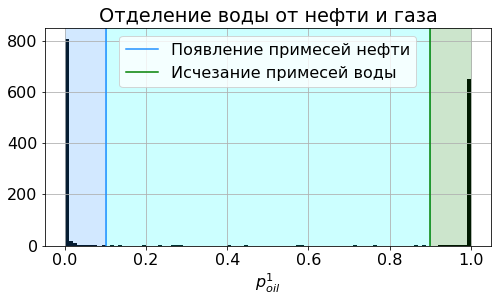
\includegraphics[width=0.8\textwidth]{TA/histogram_1.png}
\caption{Распределение значений вероятностей точек не попасть в водяной кластер. Видно, что разделение сильно бимодальное - про большинство точек мы можем с уверенностью сказать, в какой фазе они находятся; но присутствуют и точки между прямыми линиями - им мы присваиваем оценку фазового состава вода+нефть.}
\label{fig:histogram_1}
\end{figure}
\par
Аналогичная процедура проводится для модели 2 (отделение нефти от газа). Задаются пороги $thr_{oil}^2$ и $thr_{gas}^2$ такие, что $0\leq thr_{oil}^2\leq 1$ и $0\leq thr_{gas}^2\leq 1$, при этом для существования точек смены фаз необходимо выполнение условия $thr_{oil}^2+thr_{gas}^2\geq 1$.
\paragraph{Алгоритм для модели 2}
\begin{enumerate}[label=\arabic*.]
	\item Если $thr_{gas}^2\leq p_{gas}^2$, то M = «газ».
	\item Если $thr_{oil}^2< p_{gas}^2<thr_{gas}^2$, то M = «$p_{oil}^2$\% нефть+$p_{gas}^2$\% газ».
	\item Если $p_{gas}^2\leq 1-thr_{oil}^2$, то M=«нефть».
\end{enumerate}	
\par
Гистограмма распределения значений $p_{gas}^2$ для датчика 1 показана на рис.\ref{fig:histogram_2}. Для примера указаны $thr_{oil}^2=thr_{gas}^2=0.9$. Видно, что по результату работы описанного выше алгоритма большая часть точек приобретет метку «нефть» (зеленая зона) или «газ» (красная зона), в то время как небольшое количество точек в желтой зоне будут классифицированы как смесь флюидов.

\begin{figure}[H]
\centering
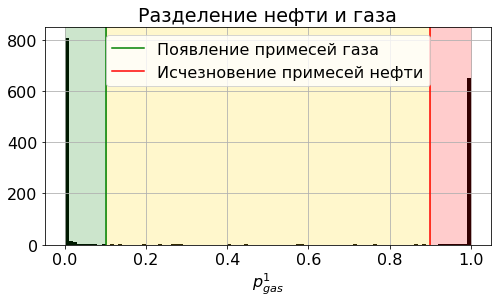
\includegraphics[width=0.8\textwidth]{TA/histogram_2.png}
\caption{Разделение нефти и газа происходит аналогично работе модели 1. Здесь распределение опять бимодальное - у большинства точек с уверенностью определяется фаза. Здесь, как и на предыдущей гистограмме, задаются отсечки между дискретной фазой и смесью флюидов.}
\label{fig:histogram_2}
\end{figure}

\par
Так как каждая точка, классифицированная как нефть, имеет как вероятность $p_{water}^1$ содержать какую-то часть воды, так и вероятность $p_{gas}^2$ содержания газа, то выбор алгоритма для модели 1 или модели 2 (то есть классификация точки как смеси «вода+нефть» либо «нефть+газ») определяется из сравнения этих вероятностей: если $p_{oil}^1>p_{oil}^2$, то используется алгоритма для модели 1, и наоборот.
\par
Полученные точки смены фаз показаны на рис.\ref{fig:sensor_1_final}(a) желтым и голубым цветами; раскраска соответствует гистограммам.
\par
На рис.\ref{fig:sensor_1_final}(b) представлена финальная разметка с оценкой фазового состава в точках смены фаз.

\begin{figure}[H]
\centering
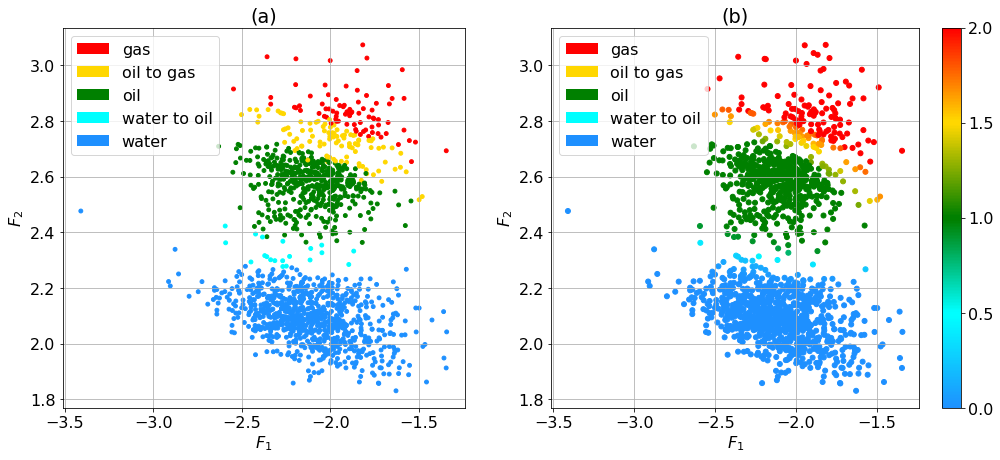
\includegraphics[width=1.0\textwidth]{TA/sensor_1_final.png}
\caption{На (a) - отделение точек смены фаз от точек, содержащих одну фазу, в соответствии с определенными ранее порогами. На (b) - то же разделение, но точкам смены фаз присвоены пропорции фазового состава.}
\label{fig:sensor_1_final}
\end{figure}
\subsection{Результаты}
\par
Финальный результат работы алгоритма – разметка с выделением точек смены фаз и оценкой фазового состава – была представлена на рис.\ref{fig:sensor_1_final}. Так как экспертная разметка была доступна только для случая однозначной классификации каждой точки как принадлежащей одному из трех классов «вода», «нефть» или «газ», то валидацию будем проводить только для первого этапа кластеризации. 
\par
После проведения разделения датасета на три кластера по построенным признакам моделью гауссовской смеси распределений получаем разметку на рис.\ref{fig:expert_comparison}(a). На рис.\ref{fig:expert_comparison}(b). показано сравнение полученной разметки с экспертной разметкой. На экспертной разметке видно, что данные разделяются на кластеры по этим признакам не так явно, как на разметке согласно предложенному методу. 
При этом основное несовпадение приходится на «нефтяной» кластер: зеленые точки попадают в облака синих и красных точек.  Это подтверждается и матрицами ошибок, рис.\ref{fig:confusion_matrices}: согласно экспертной разметке 23\% точек «нефтяного» кластера перешли в воду, а 8\% - в газ. Результаты для остальных пяти датчиков показаны в Приложении 1.

\begin{figure}[H]
\centering
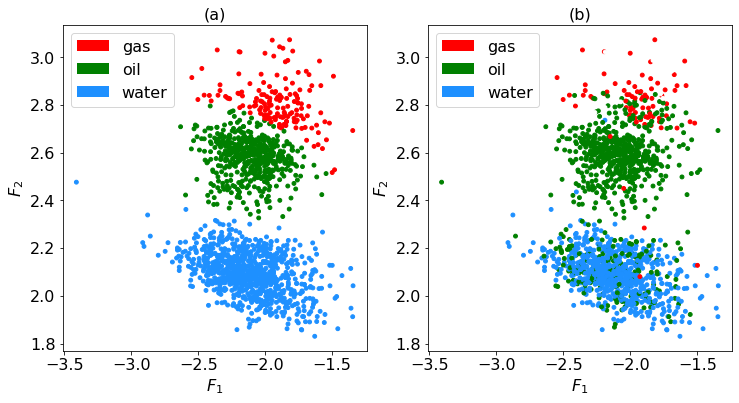
\includegraphics[width=1.0\textwidth]{TA/expert_comparison.png}
\caption{Сравнение полученной разметки (a) с экспертной (b). Синий цвет – вода, зеленый – нефть, красный – газ.}
\label{fig:expert_comparison}
\end{figure}

\begin{figure}[H]
\centering
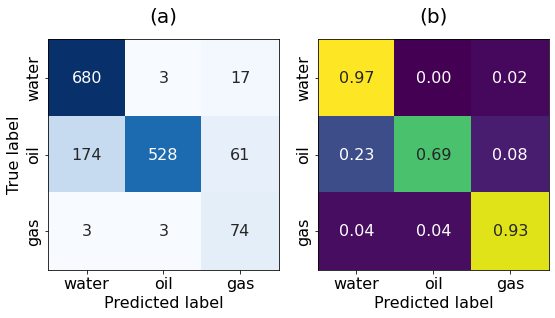
\includegraphics[width=0.6\textwidth]{TA/confusion_matrices.png}
\caption{Матрицы ошибок: (a) количество и (b) доля предсказанных значений.}
\label{fig:confusion_matrices}
\end{figure}

Одной из причин такого большого расхождения (особенно для фаз нефти и воды, которые обычно очень хорошо распознаются) является смена фаз за интервал времени цикла. В качестве примера на рис.\ref{fig:error_analysis}(d) изображен цикл, попавший в «водяной» кластер по предложенной разметке и в «нефтяной» по экспертной. Видно, что происходит смена фаз, и в начале стадии нагревания цикл действительно больше соответствует нефти, чем воде. Эти же четыре цикла показаны как точки в пространстве выбранных признаков на рис.\ref{fig:error_analysis_coordinates}.

\begin{figure}[H]
\centering
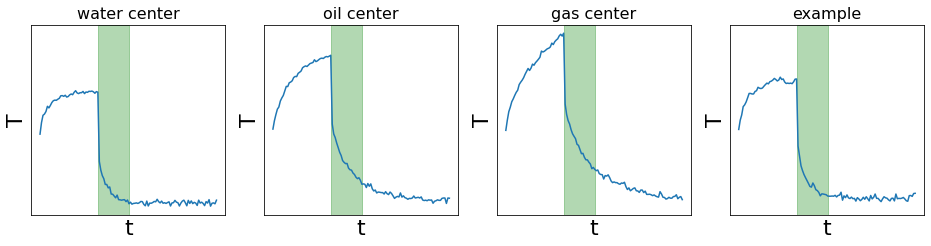
\includegraphics[width=1.0\textwidth]{TA/error_analysis.png}
\caption{Примеры циклов. Для первых трех циклов - центров кластеров - предложенная разметка совпала с экспертной. Последний цикл предложенный алгоритм определил как воду, экспертная разметка - как нефть.}
\label{fig:error_analysis}
\end{figure}

\begin{figure}[H]
\centering
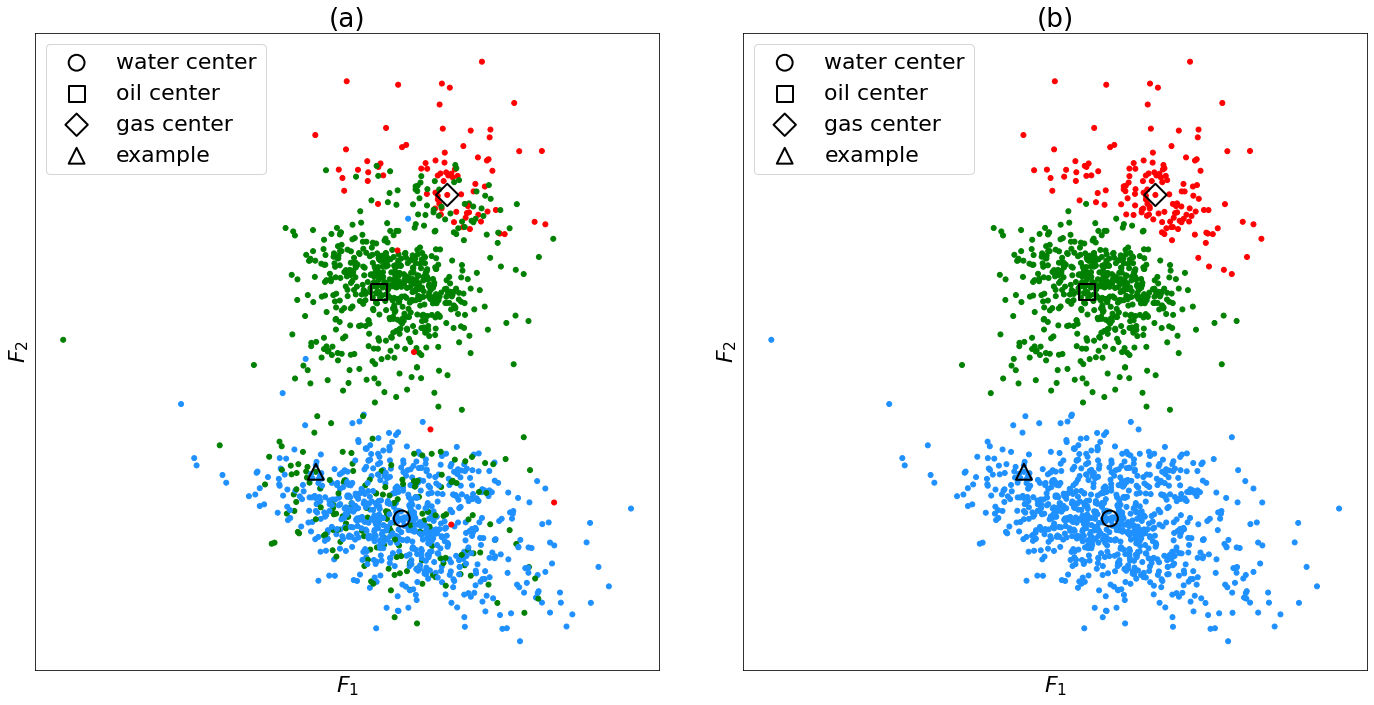
\includegraphics[width=1.0\textwidth]{TA/error_analysis_coordinates.png}
\caption{Циклы с предыдущего рисунка в пространстве выбранных координат.}
\label{fig:error_analysis_coordinates}
\end{figure}

\par
Следует отметить, что экспертная разметка проводилась на основе единственного индикатора, вычисленного на основе данных каждого цикла нагревания-охлаждения; она не является полностью ручной работой эксперта. Также без 3D-симуляции нужного уровня невозможно получить единственное решение, и в данной главе предлагается лишь еще один способ снизить неопределенность в интерпретации данных термоанемометрии. Полный цикл анализа данных должен включать в себя другие датчики и в идеале задействовать несколько различных подходов для оценки неопределенности решения; поэтому в данном случае неполное соответствие с экспертной разметкой не является проблемой.
\subsection{Обсуждение}
\par
В основе экспертной разметки, рассмотренной нами для сравнения, также лежало использование индикатора, вычисленного на основе данных каждого цикла нагревания-охлаждения (в частной беседе экспертом было указано на возможность наличия неточностей из-за неоднозначности распознавания некоторых циклов); поэтому в данном случае неполное соответствие с экспертной разметкой не является проблемой. Предложенный в данной главе новый способ нацелен на снижение неопределенности и ее оценку при интерпретации данных термоанемометрии, поскольку появляется возможность задействовать несколько различных подходов для распознавания фаз, причем в автоматическом режиме. 
\par
Оценка фазового состава должна сопровождаться и определением скоростей и массового расхода флюидов вдоль скважины. Предложенный здесь способ планируется интегрировать в эту полную задачу путем рассмотрения во взаимосвязи данных от всех шести ТА датчиков в сечении скважины, учета физики течения (например, привлечения уравнения неразрывности), траектории скважины и показаний других датчиков в сборке приборов ПГИ. Автоматизация решения этой полной задачи интерпретации на наш взгляд возможна, но потребует дальнейшего развития предложенного подхода машинного обучения без учителя. Здесь можно будет привлечь методы, разработанные в первой части работы, для выявления надежных и устойчивых индикаторов, характеризующих поток в скважине, а также учета особенностей рассматриваемых типов течений, известных из общепринятых физических моделей, полевых и лабораторных данных, опыта экспертов.
\newpage

\section{Заключение}
\par
В работе описаны алгоритмы решения двух типов задач промыслово-геофизических исследований: первый охватывает поиск событийных участков и локализацию зон притока; второй –  оценку распределения фазового состава флюидов по длине скважины. Все исследования проводились на полевых данных реальных скважин.
\par
Использованы алгоритмы машинного обучения без учителя – модель слабого контроля и кластеризация смеси гауссовых распределений; разработаны прототипы программ на языке Python. Во всех задачах в той или иной мере применялись методы цифровой обработки сигналов. При этом уже на этапе цифровой обработки сигналов при подборе параметров фильтрации и т.п. может возникнуть необходимость в машинном обучении без учителя;  для этого также возможно использование модели слабого контроля, описанной в первой части.
\par
В целом хочется отметить широкий потенциал модели слабого контроля как модели-советника по принятию решений для эксперта. Представляется, что широкий класс задач анализа данных ПГИ можно формулировать таким образом, что в качестве основы алгоритма будет выступать классификация – на два класса, на несколько или даже с присвоением нескольких меток одному объекту. При наличии достаточного количества экспертных правил (разметочных функций), позволяющих решить задачу в такой формулировке, модель слабого контроля должна выдавать надежные результаты, обоснованные теорией вероятностного машинного обучения.
\par
Важно также отметить следующее. Каждая скважина уникальна, поэтому проверка разработанных алгоритмов требует длительной и кропотливой работы по анализу их применения для все новых и новых датасетов (скважин). Более того, эта проверка неизбежно влечет за собой улучшение первоначальных алгоритмов, т.е. дальнейшую разработку и модификацию предложенных подходов.
\newline
\par
Работа выполнена при финансовой поддержке Московского научно-исследовательского центра «Шлюмберже».

\newpage

\bibliography{bibliography.bib}
\newpage

\section{Приложение}
\par
Здесь приведены результаты работы алгоритма определения фазового состава на шести датчиках одного прибора скважины T1, описанной в части 2. Далее изображения пронумерованы следующим образом:
\begin{enumerate}[label=(\alph*)]
	\item
	Изначальные данные, преобразованные в выбранных координатах. Изображения (a)-(e) демонстрируют те же данные с различной раскраской.
	\item
	Тепловая карта данных, сделанная для демонстрации плотности точек.
	\item
	Полученная дискретная кластеризация данных на три фазы: «вода» (синий цвет), нефть (зеленый цвет) и газ (красный цвет).
	\item
	Полученная кластеризация с оценкой фазового состава в точках смены фаз. Желтый цвет указывает зоны смены фаз, остальные цвета соответствуют раскраске на (c). Для демонстрации везде выбраны значения порогов $$thr_{water}^1=thr_{oil}^1=0.99,\quad thr_{oil}^2=thr_{gas}^2=0.8$$ 
	\item
	Экспертная разметка для данного датчика. Цвета соответствуют (c).
	\item
	Матрица ошибок для оценки качества кластеризации (c) в сравнении с экспертной разметкой (e). В ячейках – количество точек, соответствующих произвольной комбинации «предсказанная метка – истинная метка».
	\item
	Матрица ошибок, построенная аналогично матрице (f), но значения отнормированы по строке.
\end{enumerate}
\par
Видно, что для датчика 3 не удалось достичь хороших результатов – в выбранных координатах не видно четко выраженных кластеров.

\newpage
\begin{figure}[H]
\centering
\subfloat[]{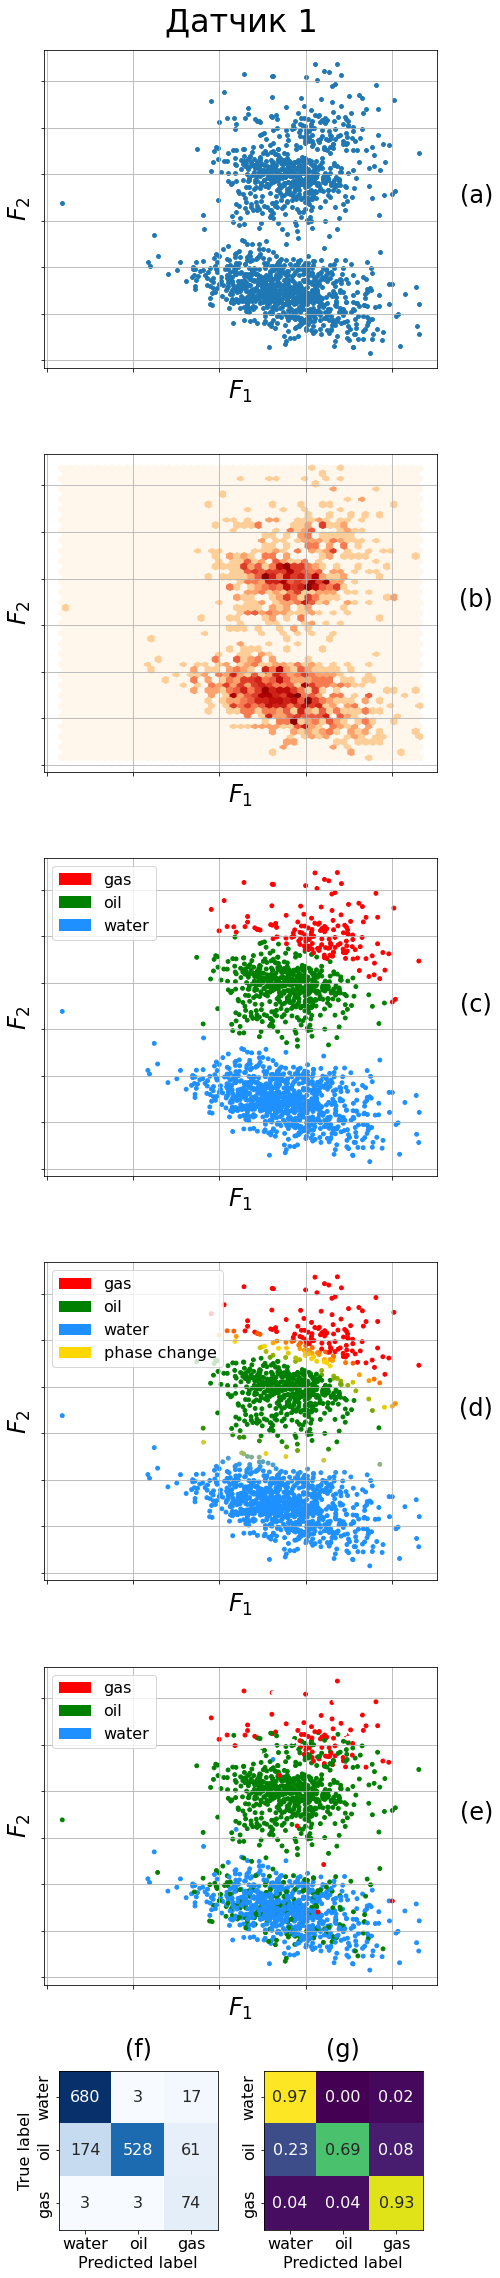
\includegraphics[width=0.3\textwidth]{TA/appendix_1.png}}
\subfloat[]{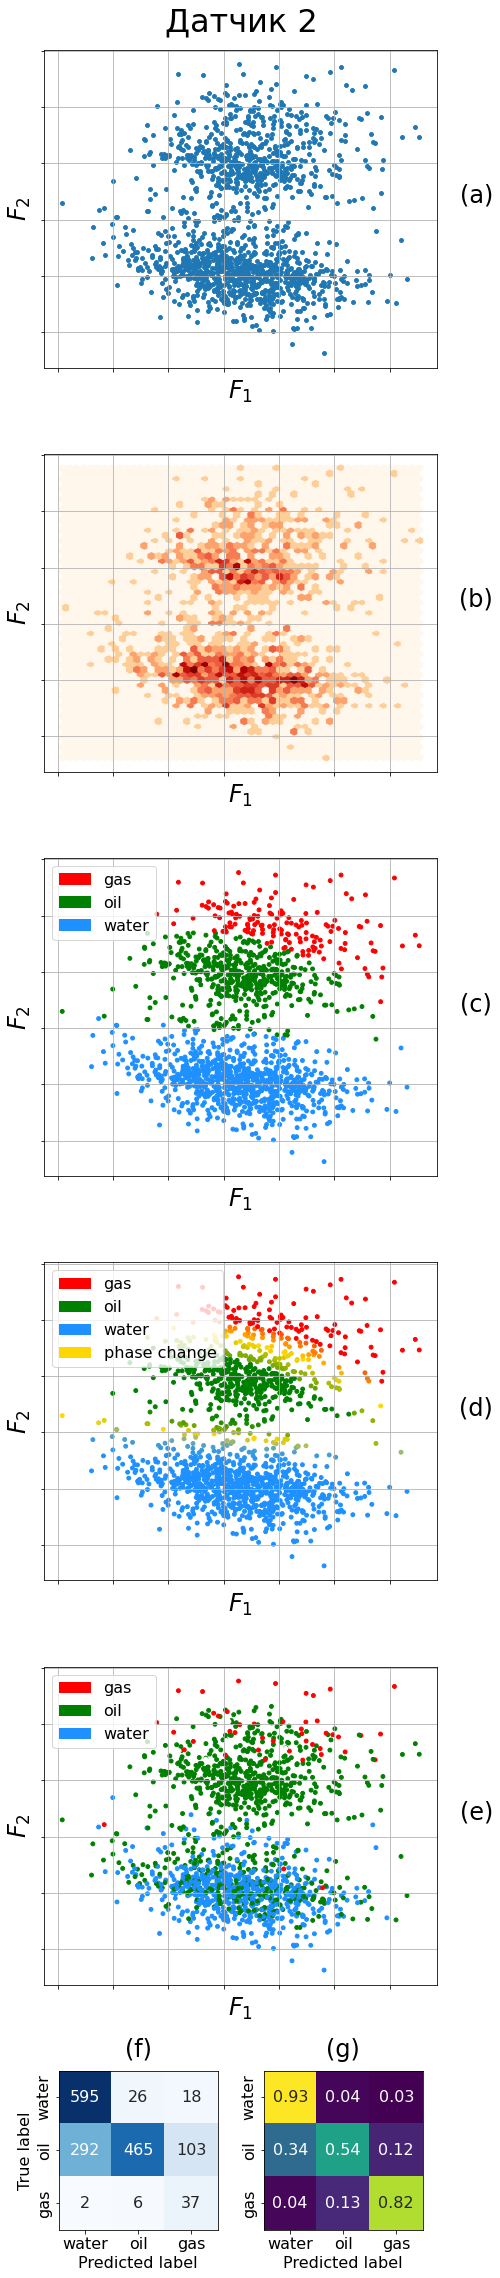
\includegraphics[width=0.3\textwidth]{TA/appendix_2.png}}
\subfloat[]{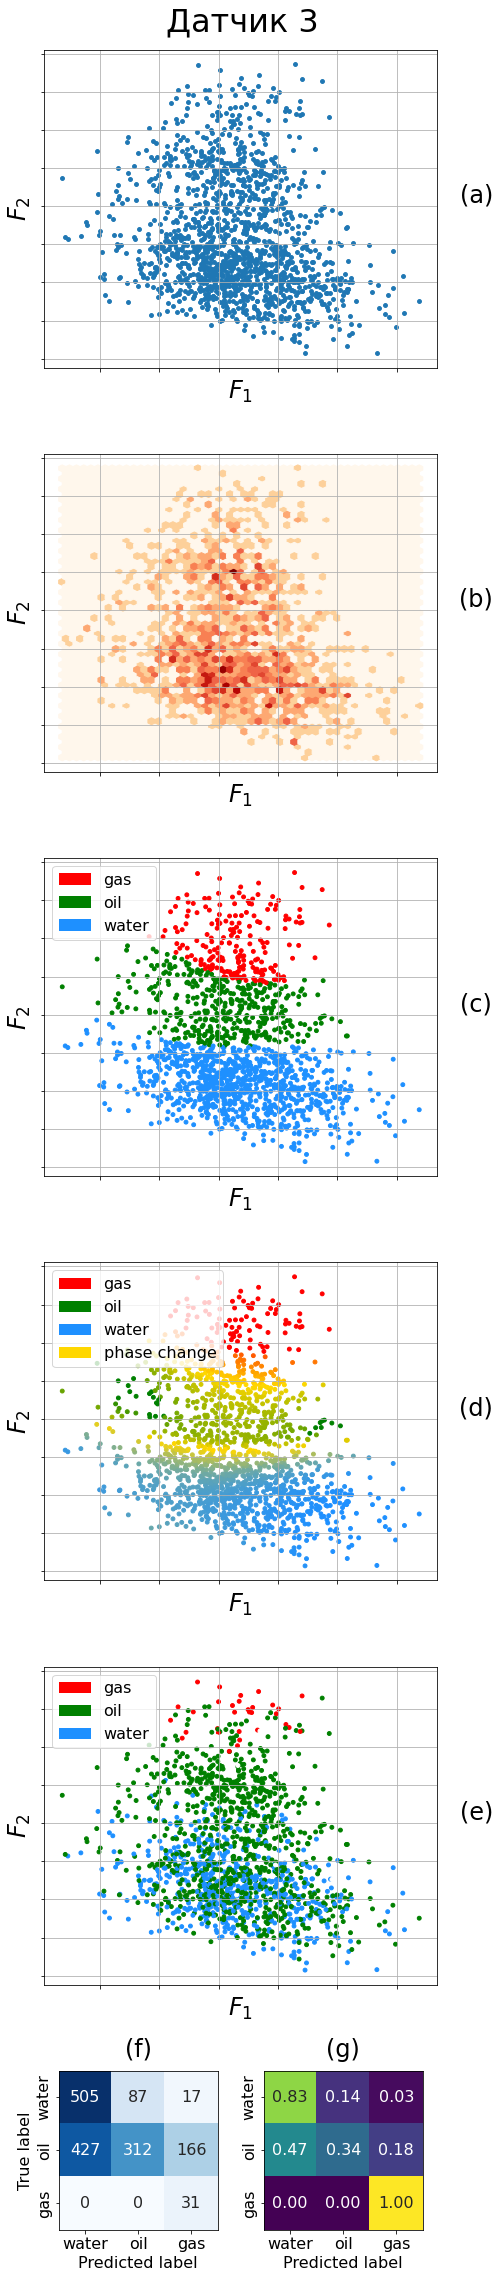
\includegraphics[width=0.3\textwidth]{TA/appendix_3.png}}
\caption{Датчики 1-3}
\label{fig:appendix_1}
\end{figure}

\newpage
\begin{figure}[H]
\centering
\subfloat[]{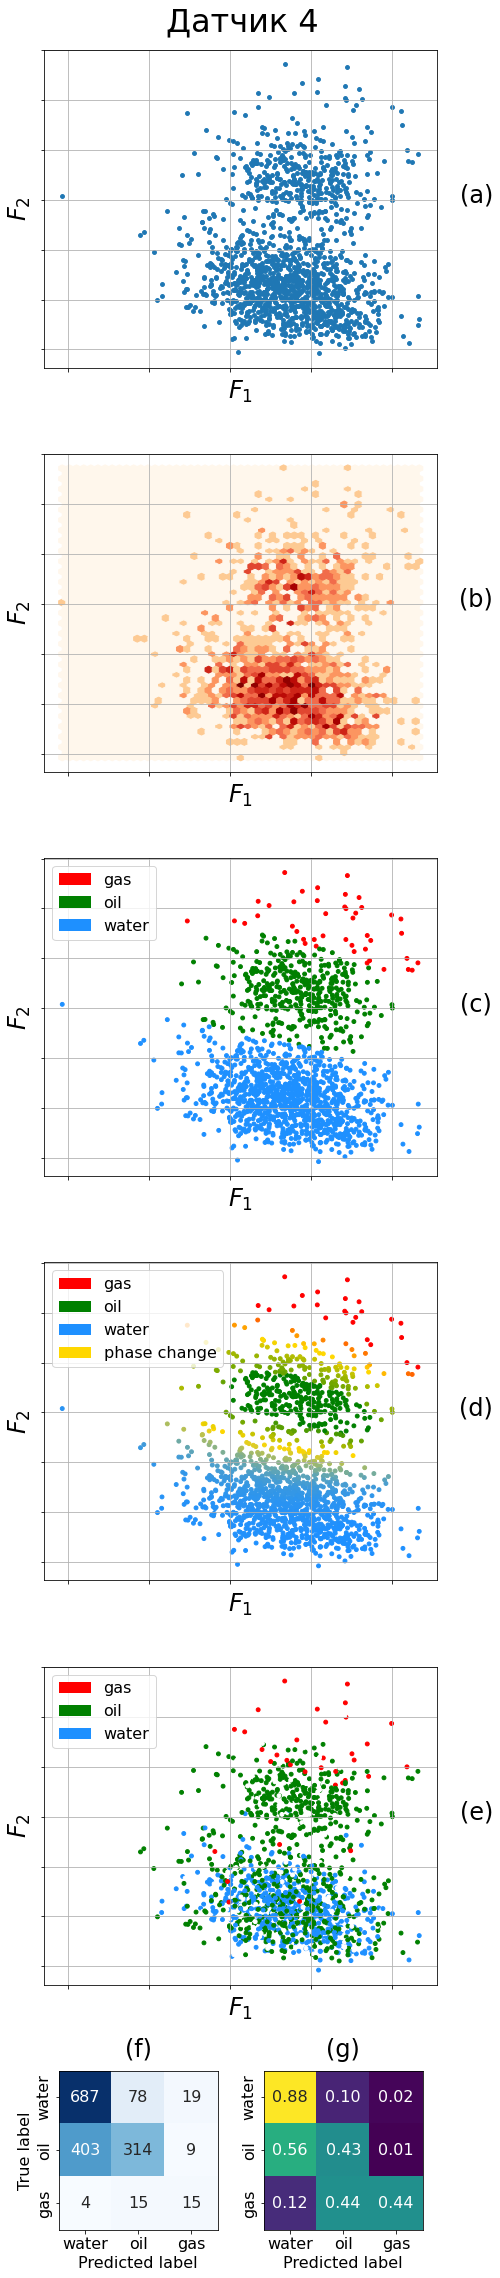
\includegraphics[width=0.3\textwidth]{TA/appendix_4.png}}
\subfloat[]{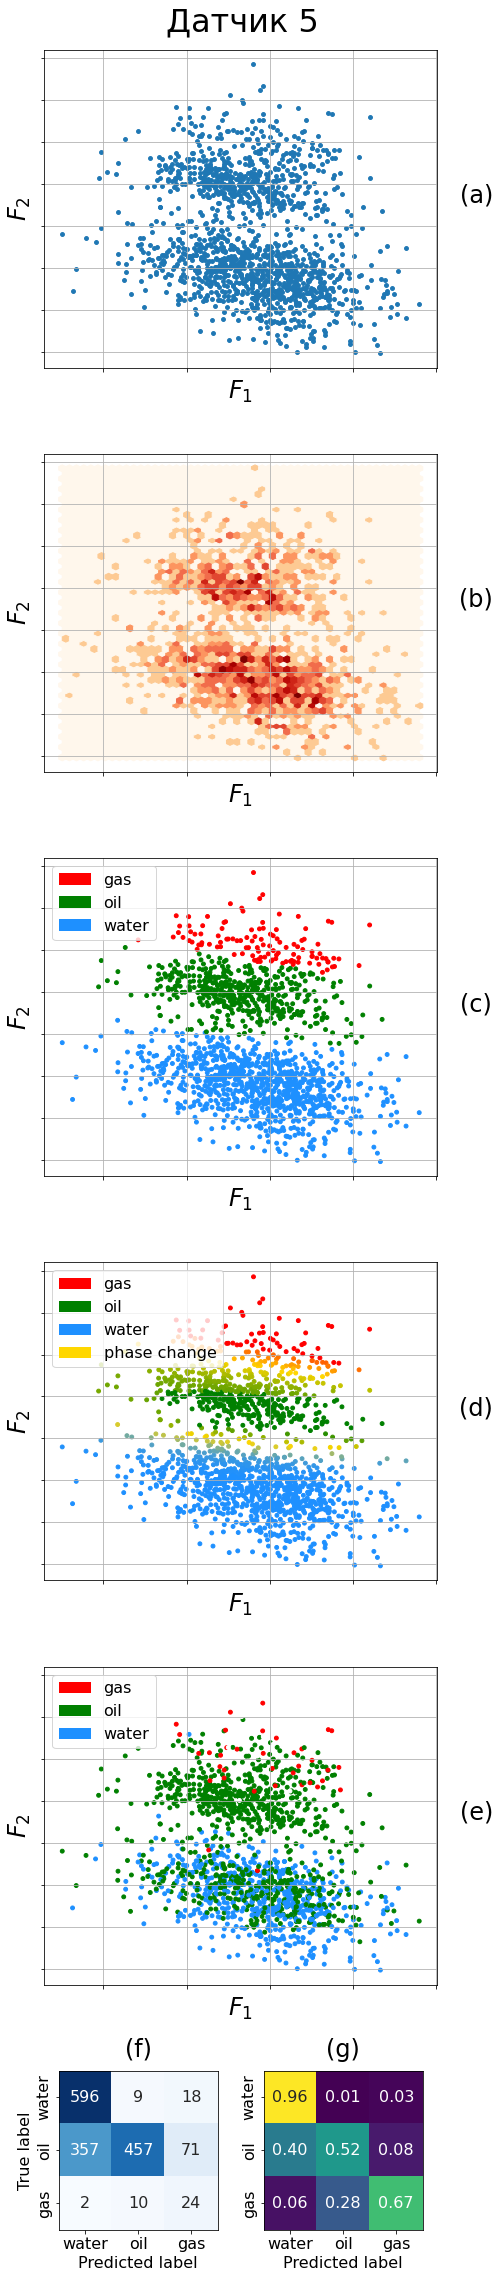
\includegraphics[width=0.3\textwidth]{TA/appendix_5.png}}
\subfloat[]{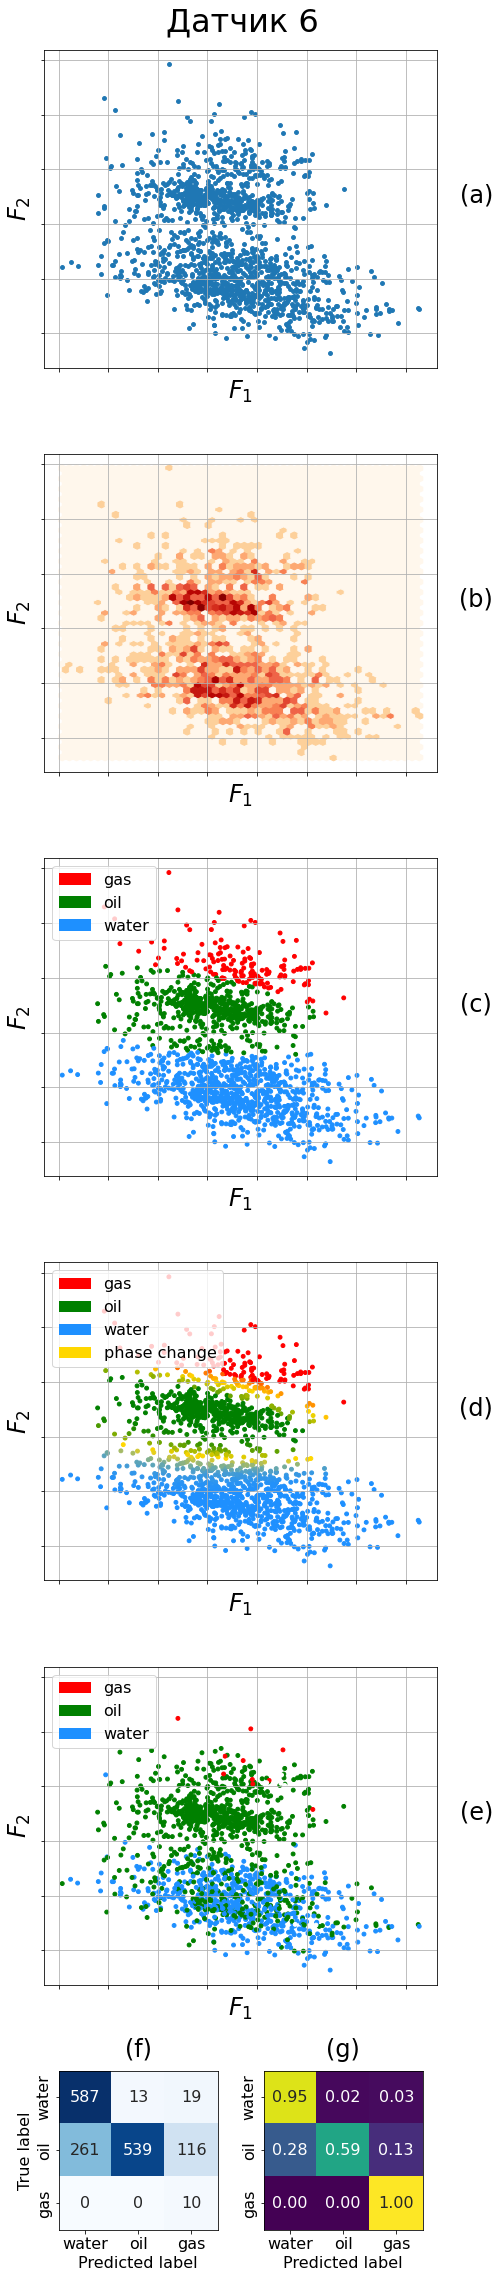
\includegraphics[width=0.3\textwidth]{TA/appendix_6.png}}
\caption{Датчики 4-5}
\label{fig:appendix_2}
\end{figure}
\end{document}